\documentclass[a4paper,10pt]{article}

%\usepackage[utf8]{inputenc} 
%\usepackage[square,sort,comma,numbers]{natbib}
%\usepackage[backend=biber,autocite=inline,style=authoryear]{biblatex}
\usepackage[backend=biber,autocite=inline]{biblatex}
\addbibresource{mybib.bib}
\usepackage{a4wide}
\usepackage{amsmath}
\usepackage{amssymb}
\usepackage{amsthm}
\usepackage{listings}
\usepackage{color}
\usepackage{enumerate}
%\usepackage{IEEEtrantools}
%\usepackage[redeflists]{IEEEtrantools}
\usepackage{verbatim}
\usepackage{graphicx}
\usepackage{subcaption}
\usepackage[section]{placeins} %no trans-sectional figures!

\usepackage{lipsum}

% Basic data
\newcommand{\N}{\mathbb{N}}
\newcommand{\C}{\mathbb{C}}
\newcommand{\ASSIGNMENT}{2}
\newcommand{\B}{\{-1,1\}}
\newcommand{\E}{\mathbf{E}}
\newcommand{\F}{\mathbb{F}}
\newcommand{\Inf}{\textbf{Inf}}
\newcommand{\I}{\mathbf{I}}
\newcommand{\NS}{\textbf{NS}}
\newcommand{\R}{\mathbb{R}}
\newcommand{\Z}{\mathbb{Z}}
\newcommand{\aufgabe}[1]{\item{\bf #1}}
\newcommand{\bvec}[1]{\mathbf{#1}}
\newcommand{\bv}[1]{\mathbf{#1}}
\newcommand{\ceil}[1]{\lceil{#1}\rceil}
\newcommand{\floor}[1]{\lfloor{#1}\rfloor}
\newcommand{\gt}{>}
\newcommand{\half}[1]{\frac{#1}{2}}
\newcommand{\lt}{<}
\newcommand{\tuple}[1]{\langle #1 \rangle}

\newcommand{\suftab}{\text{suftab}}

\setlength{\parskip}{1.0em}
\setlength{\parindent}{1em}

\lstset{
%basicstyle=\footnotesize,
%basicstyle=\ttfamily\footnotesize,
%basicstyle=\ttfamily\small,
%basicstyle=\ttfamily\scriptsize,
frame=single,
numbers=left,
%numbersep=5pt,
numberstyle=\tiny,
showspaces=false,
showstringspaces=false,
tabsize=2,
breaklines=true,
%escapeinside={#*}{*#},
%escapeinside={*\&}{\&*},% if you want to add LaTeX within your code
%mathescape=true,
%language=C++
}

\theoremstyle{definition}
\newtheorem{mydef}{Definition}[section]

\theoremstyle{remark}
\newtheorem{remark}{Remark}

\theoremstyle{plain}
\newtheorem{thm}{Theorem}[section]
%\newtheorem{thm}{Theorem}[mydef]
\newtheorem{lemma}{Lemma}[section]
%\newtheorem{lemma}{Lemma}[mydef]

\begin{document}
\renewcommand{\thesubsection}{\thesection.\alph{subsection}}\renewcommand{\thesubsection}{\thesection.\alph{subsection}}

% Document title
\begin{titlepage}
	\centering
%    \title{Bachelorthesis about Network Propagation}
%    \author{Yiftach Kolb}
%    \date{\today}
    {\scshape\LARGE \par Bachelorthesis about Community Structure in Graphs
    \par Using Network Propagation Methods 
    \par and Applications in Protein Function Annotaions}
    \vfill
  	{\Large Yiftach Kolb \par}
    \vfill
	  {\Large Instructor\par
    Prof. Dr. Matin Vingorn 
    \par}
    {\large \today\par}
\end{titlepage}

%\begin{titlepage}
%	\centering
%    %\title{Neoropraktikumsprotoklsmuster}
%    %\author{Felix Droop, Yiftach Kolb}
%    %\date{\today}
%    {\scshape\LARGE \par Protokoll von Experiment 4
%    \par vom 20/01/2020 \par Konditionierung von Larven}
%    \vfill
%  	{\Large Gruppe 7 \par Felix Droop, Yiftach Kolb \par}
%    \vfill
%	  {\large Lehrende:\par
%    Prof. Dr. Mathias Wernet, 
%    Prof. Dr. Robin Hiesinger 
%    \par Tutoren: \par
%    Lisa Peters, Johannes Hammacher, Kai Kramm, \break Nurelhoda Abdul Muti
%    \par}
%    \vfill
%    {\large \today\par}
%\end{titlepage}

%\maketitle


%\everymath{\color{blue}}
%\everydisplay{\color{blue}} 

\section{Introduction}
%This Thesis deals with the propagation methods for clustering and community
%structure in Graphs. The original motivation is to utilize these methods on
%Protein-Protein Interaction Networks (PPI) specifically for function
%annotations.
%
%We are given an (in my case undirected) connected graph, which represents some sort of
%network structure, be it a PPI or A social network. Real world networks tend to
%have some characteristics that are clearly not random, such as the 'small world
%property' and tendency to forming hubs. 

%\lipsum[1-2]

This Thesis deals with non-negative matrices, propagation methods, clustering
and community structure in Graphs. In scientific research graphs are often used
as an abstraction of a complex interaction network. They constitute a simplified
display of the information which is easier to work with yet hopefully still
retains the essential properties of the network. When that is the case, then
insightful information about the subject of research can be gained by analysis
of the graphs which are constructed out of the row data.

In the case of an unweighted undirected graph, the vertices represent particular
units that are the subject of research, be they people, proteins or whatever;
and the edges represent some sort of close proximity or interaction that is
assumed to exist between the two edges it connects.

The direct inspiration to this thesis is the subject of function prediction 
of proteins in a protein-protein interaction network (PPI). These are graphs
where the vertices represent a particular type of protein and an edge connects
two proteins if they are found in close proximity to each other in a sufficient
portion of the samples. 

It may be the case that some of the proteins in the network are well researched
already and their function is known. We are interested to the functionality of
the unknown proteins in the network based on the known proteins and the network
structure. We assume that proteins that take place in the same function will
also cluster together in the graph as they do in practice (form protein
complexes, bonds or whatever).

We may are be interested in finding the most relevant associate of a certain
known protein that has lots of neighbors. In the terminology of propagation we
are going to search for the vertex that receives the most 'heat' from the known
protein, or in terms of random walk, it is the most frequently visited vertex,
by a random path starting from the known vertex.

One advantage of propagation methods is that they are relatively fast, in fact
in linear complexity. The typical graph can be represented as a sparse matrix
and The power method starting from any starting distribution converges
exponentially fast to the greatest eigenvector which is the stationary
distribution. There are methods that achieve that in about $O(n + m)$  ($n$
vertices, $m$ edges) complexity but that is beyond the scope of this thesis.


\section{Linear algebra primer}

\begin{mydef}
\label{def:transition}
A \textbf{Transition Matrix} is a real valued non negative square ($n^2$) matrix $A$ s.t. each of its
columns sums up to one: $$A \geq 0,\ \forall j \sum_i A_{i,j} = 1$$
$A$ acts from the left as a linear mapping:
$A:v \to A \cdot v$. In the following script we treat matrices by default
as acting from the left ($Av$). 

A transition is \textbf{positive}, designated by $A > 0$ if all its entries are positive.

A transition is \textbf{primitive} if for some $k>$ $A^k$ is positive. The same
property is called \textbf{regular} in some other sources.

A transition is \textbf{irreducible} if for every entry $A_{i,j}$ there is some $k$ such
that $A^k_{i,j} > 0$.

Equivalently it can be shown that 
A matrix $A$ is 
irreducible by if and only if it is NOT
similar by permutations matrices to a block upper triangular matrix
which means 
$
\nexists P : 
A =
P
\begin{pmatrix}
B & C \\
0 & D
\end{pmatrix}
P^{-1}
$

Where $P$ is a permutation matrix and $B, C$ are square matrices of size greater than $0$.
\end{mydef}

\begin{mydef}
\label{def:state}
A \textbf{State} is a non-negative vector $v \in R^n$ s.t $\sum_i v_i = 1$.
\end{mydef}

\begin{remark}
\label{remark:state}
If $v$ is a
state and $A$ is a transition as defined in
\ref{def:transition}, then
  $Av$ is also a state because: 
$$\sum_i(Av)_i = \sum_j v_j(\sum_k A_{j,k}) = \sum_j v_j \cdot 1 = 1$$
Also its easy to confirm by multiplying with $e_i$, that if $Av$ is a state
for every state $v$ 
each column $A e_i$ must sum to $1$.
Therefore this is an equivalent definition for a transition.

If $A$ is a transition and $x,y$ are two states such that
$x \leq Ay$ then $x=y$.
\end{remark}

\begin{mydef}
\label{def:abs}
Given $A \in \C^{n \times n}$ We let $|A| \in \C^{n \times n}$ be the resulting
matrix from applying $|\cdot|$ element wise. Given a vector $v \in \C^n$ we let
$|v| \in \C^n$ the corresponding non-negative vector.

We also let $A \gt 0, v \gt 0$ mean that it holds coordinate wise. 
\end{mydef}

Here is a very useful lemma for non-negative matrices which we will need later:
\begin{lemma}
\label{lem:eqal_by_vector}
Let $0 \leq A \leq B \in \R^{n \times n}$ 
and let $0 \lt v \in \R^n$.
If $Av = Bv$ then $A = B$.
\begin{proof}
Trivial.
\end{proof}
\end{lemma}

\begin{remark}
\label{remark:abs}
If $u \in \C^n$ is on the unit circle and $T$ a transition then
$|u|$ is a state, meaning $\||u|\|_1=1$, so $T|u|$ is also a state 
so $\|T|u|\|_1=1$.

We have (component-wise) $|Tu| \leq T|u|$. If $T>0$ and $u$ has negative or
non-real entries, then this inequality must be strict and
then $\|Tu\|_1 \lt \|T|u|\|_1 = 1$.
\end{remark}

\begin{lemma}
\label{lem:exist1}
If $T$ is a transition, then
there is a state $u$ such that $Tu = u$.
\begin{proof}
Because the columns of $A$ all sum to $1$, the columns of $A-I$ all sum to $0$.
Therefore $(1,1, \dots, 1)$ is an (left) eigenvector of the rows with eigenvalue $1$.
Therefore there is also some real (right) column eigenvector with eigenvalue $1$. 
(Also it follows from the Brouer fixed point theorem because $T$ maps the $l_1$
sphere to itself).

Let $u \in R^n$ be such vector: $Au=u$. Let $u = u^+ + u^-$ such that $u^- =
\min(u_i,0)$ and the other one defined similarly for the non-negative components.

Because $A$ is non-negative $A(u^+) \geq (Au)^+ \geq 0$,
and $A(u^-) \leq (Au)^- \leq 0$.

From $A$ being
non-negative and $(Au)^+ + (Au)^- = Au = u = u^+ + u^-$
And also $(A u)^+ = (u)^+$, so we must have $Au^+ \geq (Au)^+ = u^+$ 
(component wise). But if we had a strict inequality we would get:
$\|A(u^+/\|u^+\|_1)\|_1 > 1$ which is a contradiction to $A$ being a transition
matrix.

Then $A u^+ = u^+, A u^- = u^-$ and one of them must be non-zero. It follows
that $A$ has a non-negative eigenvector with eigenvalue $1$ (one of $u^+, -u^-$
which is non-zero). If we $l_1$-normalize that eigenvector it becomes a state.
\end{proof}
\end{lemma}


\begin{lemma}
\label{lem:uniq1}
If a transition $A \gt 0$ (or primitive)
, then it has exactly
one eigenvector $v$ with eigenvalue $1$ and in addition it can be chosen so that $v > 0$
Any for any other eigenvalue
$\lambda$ it holds that $|\lambda| \lt 1$.

If $A$ is just irreducible then then again $v>0$ and is unique but there may be
additional eigenvalues on the unit circle.

\begin{proof}
Let $A \gt 0$ be a transition. We already know that there exists at least one such eigenvector.
Let $u,v$ s.t $Au=u, Av=v$. 
We can assume these are real vectors because $A$ has only real entries.
Therefore we can choose $u,v$
to be states as we have already proven above.

Then let $w=u-v$. So $Aw = A(u-v) = u-v = w$. 
And $\sum_i w_i = 1 - 1 = 0$ by choice of $u,v$.

Like before $Aw^+ = w^+, Aw^- = w^-$
and because $w \neq 0$ but sums up to $0$, both $w^+, -w^- > 0$.
Because $w^-$ is non zero exactly on entries where $w^+$ is zero and vice versa, 
each of them must have at least one $0$ entry (and one none zero). But because
$A$ is strictly positive and $w^+$ is non-negative, $Aw^+$ must have ONLY
positive entries, contradicting $Aw^+ = w^+$. It follows then that $u-v=0$ is
the only possibility, hence the eigenvector with $1$ as eigenvalue is unique.

Suppose there is $Aw = \lambda w$ where $| \lambda|=1$. Choose $w$ so it is
$l_1$-normalized. Then $|w| = |Aw| \leq A \cdot |w|$ If $w$ has any negative or
complex coordinantes, then $|Aw| \lt A|w|$ and therefore 
$1 = \| |Aw| \|_1 \lt \|A|w|\|_1 =1$, a contradiction. Therefore there cannot be
any other eigenvalues on the unit circle.

Extending this for primitive matrix is easy because for some sufficiently big
$k$ $A^k \gt 0$. 

To prove the uniqueness of the $1$-eigenvector for the irreducible case, we have
$(\forall k \in \N) A^kw^+ = w^+$ and from that with some more work left undone
it follows that $w^+ > 0$ or
$w^+ = 0$.
\qedsymbol

\end{proof}
\end{lemma}

\begin{remark}
\label{remark:rhoisone}
The lemmas and theorems in this section are phrased in term of transitions. They
hold true in the more general case of positive/non-negative
linear transformations and one just replaces $1$ with the \textbf{spectral
radius} $ \rho = \rho(A)$.

In general a non-negative linear transformation has a \textbf{spectral radius}
$\rho = \rho(A)$ which is the absolute value of its greatest eigenvalue. In the case of
positive maps there is a unique single eigenvector with $\rho$ as the unique
greatest eigenvalue and so forth \dots. When we deal with a transition map,
lemma \ref{lem:uniq1} guaranties 
it has a spectral value of $\rho(A) = 1$.
\end{remark}

\begin{thm}
\label{thm:transition_ev}
Let $T$ be a positive (or primitive) transition. Then 

1. $1$ is the greatest eigenvalue
of $T$ and it has one unique eigenvector which is also positive,
so there exists a unique stationary state.

2. All the other eigenvalues have absolute value strictly less than $1$.

3. For every state $u$, $T^ku$ converges to the stationary state $\pi$.
In particular the columns of $T^k$ converge to $\pi$.

\begin{proof}
1 and 2. We already know.

3. There is a Jordan decomposition $T = PJP^{-1}$, such that $J$ is a Jordan
matrix, $J_{1,1} = 1$ and the rest of the main diagonal $|J_{i,i}| <1$.
So now the convergence is clear $J^k \to (e_1 | 0 \dots | 0)$.
For the matrix $P$ it must hold that $P = (P_1| \dots| P_n)$ and $P_1$ is the column 
eigenvector of $T$ corresponding to $1$ which we are free to $l_1$ normalize 
and the first row of $P^{-1}$ is the
left eigenvector corresponding to $1$ and so force \dots.

Some more work or literature check should confirm that $T^k \to (v|v\dots|v) = V$.
Then one can verify $Vu = v$ for any state $u$.
\end{proof}
\end{thm}

\begin{thm}
\label{thm:transition_irr_ev}
Let $T$ be an irreducible positive (or primitive) transition. 
Then:

1. Then $1$ is the greatest eigenvalue
of $T$ and it has one unique eigenvector which is also positive,
so there exists a unique stationary state.

2. If there are other other eigenvalues on the unit circle then their algebaic
multiplicity is equal their geometric multiplicity.

3. For every state $u$, the \textbf{Cesaro sums} 
$\frac{1}{n}\sum_{k=1}^n T^ku$ converge to the stationary state $\pi$.

\begin{proof}
1 We already know.

2. There is a Jordan decomposition $T = PJP^{-1}$. such that $J$ is a Jordan
matrix, $j_{1,1} = 1$ and the rest of the main diagonal $|J_{i,i}| \leq 1$.

If we had a Jordan block of size greater than $1$ for an eigenvalue $\lambda$,
Then on the superdiagonal of $J^k$ we would have $k \lambda$. If $|\lambda| =1$
then $J^k$ and hence $T^k$ would be unbounded, but that is impossible since
$T^k$ is a transition. If follows that all eigenvalues on the unit circle must
be semi simple (alebgaic multiplicity equals geometric).

3. For the convergence, it follows from calculations on the Jordan blocks, which
I omit. See \textcite{meyer2000matrix} or \textcite{serre2010matrices}
for rigorous proof.
\end{proof}
\end{thm}

What differs irreducible non-primitive matrices from primitive is
that they are periodical on their eigenvectors with complex eigenvalues
on the unit cycle. There is, in fact a wonderful theorem from Wielandt which
characterizes these Matrices:

\begin{thm}[Wielandt (1950)]
\label{thm:wielandt}
Let $A,B \in \C^{n \times n}$ such that $A \geq 0$ is irreducible and $|B| \leq
A$ (component-wise). Then $\rho(B) \leq \rho(A)$.
If $\rho(B)=\rho(A)$ then $|B|=A$, $B$ has an eigenvalue of the form $\mu =
\rho(A)e^{i \phi}$ and:

\begin{equation}
\begin{aligned}
\label{eq:wielandt1}
B &= 
e^{i \phi}DAD^{-1} \\ 
\text{where } D \text{ has the form:}\\
D &= 
\begin{pmatrix}
e^{\theta_1} & & & \\
& e^{\theta_2} & & \\
& & \ddots & \\
& & & e^{\theta_2}
\end{pmatrix}
\end{aligned}
\end{equation}

And conversely any $B$ of the form \ref{eq:wielandt1}
has $\rho(B) = \rho(A)$, $|B|=A$ and $\mu$ is an eigenvalue of $B$ which
corresponds to the eigenvalue $\rho(A)=|\mu|$ the greatest eigenvalue of $A$.

\begin{proof}
To see a rigorous proof I suggest \textcite{meyer2000matrix}.

The keys for proving this theorem are:
First WLG assume $A$ is a transition. This is possible because we may replace
$A$ with $AW^{-1}$, and $B$ with
$BW^{-1}$, where $W$ is the diagonal matrix that has the column-sums of $A$.
Since $A$ is irreducible it cannot have a column or a row that is all $0$
so this diagonal is positive $W$ is indeed invertible and later we can cancel out the
$W$'s and return to the general case.

Let $v$ be the $\mu$-eigenvector $Bv = \mu v, \|\mu|=1$ and choose it so that 
$\|v\|_1=1$.

Then 
\begin{equation}
|v| = |\mu v| = |B v| \leq |B| |v|
\leq A |v|
\end{equation}

Since $A$ is a transition by remark \ref{remark:state} $A|v|=|v|$. Since $A$ is
irreducible and $A|v| = |v|$ we must have by \ref{thm:transition_irr_ev} that
$|v| \gt 0$, and then by
lemma \ref{lem:eqal_by_vector} $A = |B|$ so that proves the first part.  

Now let $w = v / |v|$ (component-wise division) and let 
\[D = \text{diag}(w) = 
\begin{pmatrix}
e^{\theta_1} & & & \\
& e^{\theta_2} & & \\
& & \ddots & \\
& & & e^{\theta_2}
\end{pmatrix}
\]

Then $v = D|v|$, $|v|=D^{-1}v$ and we have:

\begin{equation}
\label{eq:wielandt1proof}
\begin{aligned}
A|v| &= |v| = D^{-1}v = \\
&= D^{-1} \mu^{-1} B v = \mu^{-1} D^{-1} BD|v|
\end{aligned}
\end{equation}

We know already that $|v| \gt 0$. If 
$C := \mu^{-1} D^{-1} BD$ contains any negative or complex entries, then
\ref{eq:wielandt1proof} cannot hold. It follows that
\[
A = C = \mu^{-1} D^{-1} BD 
\]

This proves the harder direction of the claim, the other direction is easy \qedsymbol.

\end{proof}
\end{thm}

The amazing consequence from \ref{thm:wielandt}:

\begin{thm}[Corollarly]
\label{thm:wielandt2}
If $A$ is irreducible transition with $h$ 
eigenvalues on the unit circle then its eigenvalues are exactly the $h$th unit roots
$\lambda_k = e^{2 \pi i k /h}, k = 0 \dots n-1$ and $A$ is similar to $\lambda
A$ by a diagonal matrix for any such eigenvalue.

\begin{proof}
Use theorem \ref{thm:wielandt} with $B=A$. If $|\lambda|=1$ is an eigenvalue
then $A = \lambda D A D^{-1}$. Since similarity doesn't change the eigenvalues,
$A$ and $\lambda A$ must have the same eigenvalues with the same multiplicity.
Since $1$ is a simple eigenvalue of $A$ and hence of $\lambda A$, and its
corresponding eigenvalue $\lambda$ is simple in $\lambda A$ and therefore in $A$
as well.

The matrices $\lambda_k A$, $k=0 \dots h$ are all similar, with $\lambda_0 = 1$
and $|\lambda_k| = 1, k=0 \dot h-1$ all simple eigenvalues. The only way for this to hold is if
$\{\lambda_k\}_0^{h-1}$ form a multiplicative group of order $h$ on the unit
circle, in other words, the eigenvalues are exactly all the $h$th unit roots. 
\end{proof}
\end{thm}

\begin{remark}
\label{remark:wielandt_cyclicity}
If $A$ is irreducible transition with exactly $h$ 
eigenvalues on the unit circle then $h$ is called the \textbf{period} of $A$.
$A \geq 0$ is primitive if and only if it is irreducible and aperiodic ($h=1$).

If $\omega = e^{2 \pi i /h}$ then \ref{thm:wielandt2} shows that $A = \omega D A
D^{-1}$. So if $\lambda$ is any eigenvalue not necessarily on the unit circle,
then $\omega \lambda$ is also an eigenvalue with the same multiplicity and
rotation with $\omega$ is an automorphism on the eigenvalues.

We may choose $D$ so that $D[1,1]=1$. If we reindex the dimension we can make
$D$ look like 
\[
D = [D_0 | \omega D_1 | \dots \omega^{h-1} D_{h-1}]
\] So Indexes corresponding to the same phase of the period appear sequentially.


Then use the identify $\forall k D^hA^{k} = A^k D^h$ and the fact that $A$ is
irreducible to show that $D^h = I$. Then use the identity $\omega DA = AD$ to
show that in the new indexing $A$ has the following periodical block structure
($0$ on the main diagonal):

\[
A = 
\begin{pmatrix}
0 & M_1 & 0 & \dots & 0 \\
0 & 0 & M_2 & 0 \dots & 0 \\
 &  & \ddots & \ddots & &  \\
0 & \dots & 0 & 0 & M_{h-1} \\
M_h & 0 & \dots & 0 & 0 
\end{pmatrix}
\]
\end{remark}


Now we will just present the Perron-Frobenius theorems. The main parts that are
important to our work have appeared in the previous theorems.

\begin{thm}[Perron-Frobenius \cite{meyer2000matrix}]
\label{thm:perron1}


Let $0 \lt A \in \R^{n \times n}$ with spectral radius $\rho := \rho(A)$, then the following are all true:
\begin{itemize}
\item{} $\rho \gt 0$
\item{} $\rho$ is a simple root of the characteristic polynomial of $A$,
in other words its algebraic multiplicity is $1$.
\item{} $(\exists v > 0) Av=\rho v$
\item{} If $Au = \lambda u$ and $\|u\|= \rho$ then $\lambda = \rho$
namely, $\rho$ is the unique eigenvalue on the spectral circle.
\item{(Collatz-Wielandt Formula)} $\rho = \max_{x \in \Gamma} \min_{i : x_i \neq 0} [Ax]_i / x_i$
with $\Gamma = \{x | x \geq 0, x \neq 0\}$
\end{itemize}
\end{thm}

\begin{thm}[Perron-Frobenius for irreducible matrices \autocite{meyer2000matrix}]
\label{thm:perron2}

Let $0 \leq A \in \R^{n \times n}$ be irreducible with spectral radius $\rho := \rho(A)$,
then the following are all true:
\begin{itemize}
\item{} $\rho \gt 0$
\item{} $\rho$ is a simple root of the characteristic polynomial of $A$,
in other words its algebraic multiplicity is $1$.
\item{} $(\exists v > 0) Av=\rho v$
\item{} There are no additional non-negative unit eigenvectors of $A$ other than
$v$. 
\item{(Collatz-Wielandt Formula)} $\rho = \max_{x \in \Gamma} \min_{i : x_i \neq 0} [Ax]_i / x_i$
with $\Gamma = \{x | x \geq 0, x \neq 0\}$
\end{itemize}
\end{thm}


\section{More on matrices, graphs and stochastics}

A directed non-weighted graph $G$ can be uniquely represented by its
\textbf{adjacency matrix},
$A_{i,j} := 1$ if and only if there is a directed edge from $i$ to $j$ (if we
want to use it for transitioning on columns as done above). It's possible to
assign different edge weights rather than only $1$ and $0$. If the graph is
undirected each edge would be counted in both directions and the matrix is
symmetric.
Relabeling the vertices of a graph yields an adjacency matrix that is similar by
permutations ($PAP^{-1}$, where $P$ is a permutation matrix) and vice versa.

To turn $A$ into a transition, normalize each column by dividing it with
its out going rank, so let $D_{i,i} = \text{out~rank}(i)$, $T:=AD^{-1}$ is the
transition matrix of this graph (because right-multiplying by $D$ normalizes each
column by its rank).
If the graph was stochastic to begin with then the adjacency matrix as we
defined it is already column-normalized.

\begin{mydef}
\label{def:stronglyconnected}
A graph is $G$ \textbf{strongly connected} if there is a directed path form any edge
to any edge. Equivalently $G$ is strongly connected if and only if its adjacency matrix is irreducible.

We say that the \textbf{Period of a vertex} $v \in V(G)$ is the greatest common
divisor of all closed paths on $v$. If the periods of all vertices are equal
(spoiler: in the case that $G$ is strongly connected they are), we call it the
\textbf{Period of the graph} $G$.
\end{mydef}

\begin{remark}
\label{remark:periods}
If $G$ is strongly connected then the periods of all vertices are indeed equal
and its easy to prove. The corresponding adjacency matrix $A$ is irreducible so
it too has a period $h$ as defined in \ref{remark:wielandt_cyclicity} and it is
equal to the graph period (can be shown using \ref{thm:wielandt2} and
\ref{remark:wielandt_cyclicity}).

So if the graph $G$ is strongly connected and has period $1$
then the adjacency matrix is \textbf{aperiodic} and hence primitive, and vice versa. 
\end{remark}

From all the above we have seen that a Markov process can be represented in two
equivalent ways \textemdash as a transition matrix  and as the 
corresponding weighted directed graph.

If the graph $G$ is strongly connected and aperiodic, its corresponding
adjacency matrix is primitive. We know from \ref{thm:perron1} that there is a
unique stationary distribution $p$ and that the Markov converges to $p$ no
matter from which distribution it starts. We may calculate $p$ using the
\textbf{power
method} which is efficient because it can be done in a matrix-free method. 
We don't need to know the matrix itself just the dot product of it with a state
vector.

If the graph $G$ is strongly connected, then \ref{thm:perron2} assures us the
existence and uniqueness of a stationary distribution $p$. But if $G$ is not
aperiodic, the corresponding adjacency matrix is not primitive. We cannot use
the efficient power method to calculate $p$. Also the process itself doesn't
stabilize on $p$. It is periodic and cycles between the $h$ eigenvectors on
the unit circle. 

We are therefore interested to find how to convert an \text{imprimitive}
matrix (= irreducible but not primitive)
to a primitive matrix or equivalently to turn a strongly connected but periodic graph
into an aperiodic graph.

\begin{lemma}
\label{lem:1plusA}
Let $A \geq 0$ be irreducible. Then $(A + I)^{n-1} \gt 0$, and therefore $A+I$
is primitive.
\begin{proof}
Notice that the $I$ represents self loops and it absorbs all the lower powers so
if $(A^k)_{i,j} \gt 0$ for some $k \lt n$ then so is $(A+I)^{n-11}$.
Let $G := G_A$ be the corresponding graph to $A$. Then $G$ is strongly
connected. For every $i \neq j$ there is a directed \textbf{shortest path}
$\sigma$ in $G$ from $i$ to $j$. Its length must be $|\sigma| \lt n$. Otherwise
$\sigma$ would have to contain a cycle and not be of minimal length.
This shows that we have for every $i \neq j$ some $k$ sucht that $A^k_{i,j} \gt
0$ and therefore $(A+I)^{n-1} \gt 0$.
\end{proof}
\end{lemma}

The properties of irreducibility, primitiveness and positivity only depend on the
sign ($-,0,+$) of the entries and not on their size. So we use the following definition to
test matrices for these properties:

\begin{mydef}
Let $A \in \R^{n \times n}$, then its \text{binary form} is the matrix
$\beta(A) := \text{sgn}(A)$ where $\text{sgn}$ is applied element-wise.
\end{mydef}

The following trivial lemmas would help as to construct primitive transitions:

\begin{lemma}
$A$ is positive/primitive/irreducibly if
and only if $\beta(A)$ is.

Let $0 \leq \beta(A) \leq \beta(B)$.
Then If $A$ is positive/primitive/irreducibly so is $B$.

Let $0 \lt \alpha \lt 1$. If $T,S$ are transitions the so is $W=(1-\alpha)T +
\alpha S$.
If one of $S,T$ is positive/primitive/irreducible so is $W$
\end{lemma}

Let $G$ be any weighted graph and $A$ its adjacency transition matrix. Some vertices may
be unreachable from other vertices and there might not exist a single and
unique stationary distribution. A random walk on this graph is generally
dependent on the initial state.
However if we allow the possibility of 'random restart' from any state, this
graph becomes totally connected it is guarantied to have a unique stationary
distribution to which any random walk converges regardless of the initial state.

In terms of matrices, we create a positive transition matrix $W = (1-\alpha)A +
\alpha \mathbf{\frac{1}{n}} \gt 0$. Where $\mathbf{\frac{1}{n}}$ is the $n
\times n$ matrix whose entries are all $\frac{1}{n}$. The stationary
distribution is called the \textbf{PageRnak} for $G$ with restart parameter
$\alpha$. It is used to order the vertices according to their 'relevance' in the
network.


\begin{figure}[!htb]
  \centering
    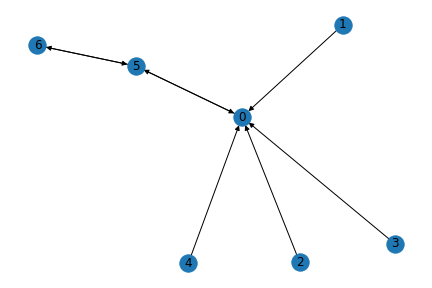
\includegraphics[width=0.55\linewidth]{directed_graph_example_unranked.png}
  \caption{This is an example of a weakly connected graph. If we start walking
  from $0$, $5$ or $6$ we can never reach vertices $1-4$. It is also not immediately
  clear which vertex $0$ or $5$ is more 'important'. While $0$ is directly
  connected to more vertices, $5$ may get more 'flow' through it since every
  path of length $2$ or more passes though it.}
  \label{fig:weaklyconnected}
\end{figure}

\begin{figure}[!htb]
  \centering
    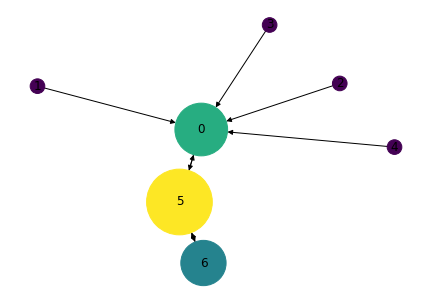
\includegraphics[width=0.55\linewidth]{directed_graph_example.png}
  \caption{The same graph with vertex size and color indicating its PageRank
  with parameter $\alpha=0.15$. We see that $5$ is ranked first, followed by
  $0$. The smaller the restart parameter, the more important $5$ will get
  because we allow for longer paths with fewer restarts.}
  \label{fig:weaklyconnectedpagedranked}
\end{figure}

\begin{figure}[!htb]
  \centering
    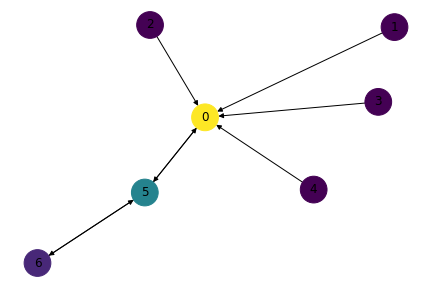
\includegraphics[width=0.55\linewidth]{directed_graph_example_tinyalpha.png}
  \caption{When the restart parameter is too large, the rank becomes almost
  uniform because the convex combination of the original graph with the
  $n$-clique graph of the restarts is weighted too heavily on the latter. It
  also shows that for high restart values $0$ becomes hotter than $5$. That is
  because paths of length $\gt 2$ (before restart) become very unlikely in this random walk.}
  \label{fig:weaklyconnectedpagedrankedbadly}
\end{figure}

\begin{figure}[!htb]
  \centering
    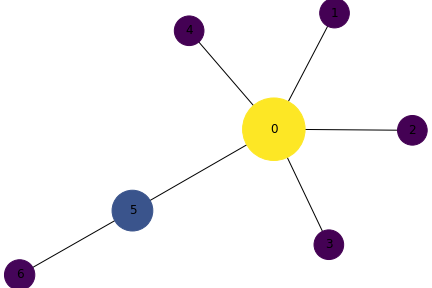
\includegraphics[width=0.55\linewidth]{undirected_graph_example.png}
  \caption{When we treat the graph as undirected and calculate the PageRanks
  ($\alpha=0.15$),
  Vertex $0$ comes this time on top. It is more central than $5$ and
  more random paths intersect it than any other vertex.}
  \label{fig:undirectedanked}
\end{figure}

The PageRank is the stationary distribution of the process when we use unbiased
restart\textemdash A restart is equally likely from any vertex.
But we want more. We want to find out what happens when we restart, for example,
always from one single vertex $u$. We think of the stationary distribution $p_u$ that 
results from such process as the heat (or flow) which propagates out of $u$.
If we take another vertex $v$ we think of $p_u[v]$ as a measure of how close $v$
is to $u$, or how much heat $u$ sends to $v$.
Note that this is not symmetric $p_v[u] \neq p_u[v]$ in general.

%(memo: add an illustration about asymmetry)

\begin{figure}[!htb]
\centering
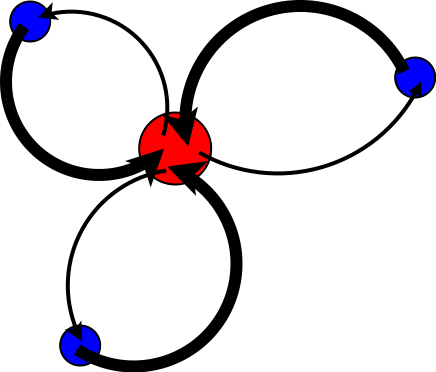
\includegraphics[width=0.55\linewidth]{diagram_star.png}
\caption{Stars have hot center because it spreads its heat on many sources,
while each of the orbiting vertices sends all its heat into the star center.
}
\label{fig:hotstar}
\end{figure}

\begin{lemma}
\label{lem:AplusP}
Let $A \geq 0$ be irreducible. Let $B \geq 0$ have a positive row (or column),
then $A + B$ is primitive.
\begin{proof}
Suppose WLG that $B_1 > 0$ (first row). Then $\forall k \gt (B^k)_1 \gt 0$.
Fix $i,j$.
Since $A$ represents a strongly connected graph, there is a path from $i
\curvearrowright 1 \curvearrowright j$ of some length $k$. So $A^k_{i,j}>0$.
Then $\forall l \geq 0 (A + B)^{k+l} \gt 0$ because we can go along this path,
then self loop $l$ times in $1$ and keep going to $j$ on that path.

So we have shown that $(A+B)^k_{i,j}$ stays positive once it becomes positive
and it always turns positive at some point by irreducibility of $A$, so that
means $A+B$ is primitive.
\end{proof}
\end{lemma}

\begin{remark}
\label{rem:AplusP}
Lemma \ref{lem:AplusP} proves that we can propagate from any arbitrary restart
group including a single vertex and the combined transition matrix will be
primitive if the adjacency matrix $A$ is strongly connected.

Let $q$ be a state column vector for example $e_1$ and let $Q = (q | q | \dots | q)$.
So $Q$ has a positive row and therefore $(1-\alpha)AD + \alpha Q$ is a primitive
transition.

Also worth noting that if $x \geq 0$ is any transition, then $Qx = q$.
\end{remark}

If $A$ is the adjacency matrix of $G$ we defined the transition $T = AD^{-1}$.
We define the transition matrix with restart parameter $\alpha$ and bias $q$ as
\[
T_{\alpha, q} :=
(1 - \alpha)T + \alpha Q
\]

This matrix has a unique stationary distribution $p$ so
And use \ref{rem:AplusP}:

\[
p = Ip
= [(1 - \alpha)T + \alpha Q]p =  (1 - \alpha)Tp + q 
\]

We can rearrange it now

\begin{equation}
\label{eq:uninvertedstationary}
(I - (1 - \alpha)T)p = \alpha q
\end{equation}

We want to invert the matrix in \ref{eq:uninvertedstationary} and use the
following lemma to justify it (Th proof is easy. See for example
\textcite{serre2010matrices}):

\begin{lemma}
\label{lem:invertible}
Let $X$ be a contracting matrix, Then $(I-X)$ is invertible and the power sum of
$X$ converges to it:
\[
(I - X)^{-1} = \sum_{k=0}^{\infty} X^k
\]
\end{lemma}

So now we may apply lemma \ref{lem:invertible} on equation
\ref{eq:uninvertedstationary} because $(1-\alpha)A$ is contracting, and we have:

\begin{equation}
\label{eq:diffkernel}
p = \alpha [I - (1 - \alpha)T]^{-1} q := K q = 
\alpha \sum_{k=0}^{\infty} (1 - \alpha)^k T^k
\end{equation}

$K$ is called \textbf{diffusion kernel} of $T$ with parameter $\alpha$
It turns out that $K$ itself is a transition because it maps the
arbitrary transition $q$ to the transition $p$. In addition, $K \gt 0$ because
of \ref{eq:diffkernel}.

What about the eigenvectors and eigenvalues of $K$?
If a matrix $A$ is invertible then $Av = \lambda v \iff A^{-1}v = \lambda^{-1}$.
For any matrix $Av = \lambda v \iff (I + A)v = (1+\lambda)v$.

It turns out then that $T$ and $K$ have the same eigenvectors and if $Tv=\lambda
v$ then $K v = \alpha [1 - (1 - \alpha) \lambda]^{-1} v$. And in particular if it
turns out that all the eigenvalues are real (spoiler- they are), then they have
the same order as eigenvalues of $K$ or $T$ for the same eigenvector.
In particular we see that the choice of $\alpha$, the restart parameter, NEITHER 
changes the eigenvectors NOR does it change the order of the eigenvalues.

To sum up the important facts that we would need later:

\begin{thm}
\label{thm:AKTcharacteristics}
Let $G$ be strongly connected undirected graph. Let $A$ be its adjacency matrix
and $D$ the diagonal matrix which has the ranks of the vertices on its diagonal.
Let $T = A D^{-1}$, let $0 \lt \alpha \lt 1$ and 
$K = \alpha [I - (1 - \alpha)T]^{-1}$. Then the following are all true:

\begin{itemize}

\item{}
$A \geq 0$ is symmetric therefore its eigenvalues are all real.

\item{}
$T = AD^{-1} = D^{1/2}[D^{-1/2}AD^{-1/2}]D^{-1/2}$ is similar to $A$. Therefore
it has the same eigenvalues as $A$, which are all real:
$\lambda_1 \geq \dots \lambda_n$.

\item{}
There exists for all $0 \lt \alpha \lt 1$ the invertible matrix: 
$K := \alpha \sum_{k=0}^{\infty} (1 - \alpha)^k T^k = \alpha [I - (1 -
\alpha)T]^{-1}$.
$K \gt 0$ is a transition. It has the same eigenvectors as $T$ and their
corresponding eigenvalues are all real and they have the same order as the
corresponding eigenvalues for $T$ have.
\end{itemize}
\end{thm}

Finally as a side note the name diffusion kernel originates from the heat
equation which associated with the graph, considering the graph 
as perfectly insulated system.
We won't get deeper into that at this time.

%The Equation looks something like this: Let $L = D - A$, the \textbf{Laplacian
%Matrix}. Let $\gamma \gt 0,$ and $0 \lt p_0 \in \R^n$ 

\section{A naive yet not useless propagation method for clustering a graph}

\begin{mydef}
\label{def:influence}
Let $G$ be a strongly connected graph and $K$ the diffusion kernel as defined in
\ref{lem:invertible}, end let $u,v \in \{1 \dots n\}$ be two vertices and $e_u,
e_v \in \R^n$ their corresponding index vectors.

$p_u := K e_u$, the stationary distribution with random restart from $u$,
is called the \textbf{influence vector} of vertex $u$. We say that $p_u[v]$
is the \textbf{influence of} $u$ on $v$.
\end{mydef}

A $p_u$ is a measure of how 'heat' which is pumped into $u$ propagates in the graph.
When we try to cluster the graph, it is natural to think that If vertex $v$
is the top receiver from $u$, namely $v = \text{argmax}(p_u)$ then maybe these 2
belong in the same cluster.

Informally we say that a vertex is 'hot' or 'cold' if it has a high (hot) or low
(cold) PageRank. Remember that the PageRank is the unbiased stationary distribution
$p = K \cdot (1/n, \dots, 1/n)^t$.

So when we start clustering a graph, I suggest that it makes sense to pick up a
cold vertex and associate it with the vertex to which it sends most of its heat.
If we start from a hot vertex, it usually has many neighbours and it doesn't
send allot of heat down a single vertex.

The algorithm works as follows:

\begin{lstlisting}
function coolWarmClustering(G, k)
  # Input G = (V,E) : a directed strongly connected graph.
  # Input m : The desired number of clusters
  K <- diffusion_kernel(G)
  H <- Disconnected_undirected_graph_on(V) # each vertex starts in its own cluster 
  p <- pageRank(G)
  vlist <- arg_sort(p) # vertex-list sorted up by PageRank 
  While |connected_components(H)| > k do
    x <- vlist.pop() # take the coldest remaining vertex and remove it from the
                      # list
    p_x <-K * e_x # Influence vector of x
    y <- argmax(p_x)
    H.add_edge(x,y)
  return H
\end{lstlisting}

The algorithm clusters the vertices by constructing a new graph on the same
vertices, successively joining vertices. It picks the coldest remaining vertex
and joins it with the vertex to which it propagates the most heat.

In every iteration of the algorithm adds an edge, which either reduces the
number of connected components by $1$ or keeps it unchanged. Because $G$ is
strongly connected algorithm will reduce the number of connected
components in $H$ until it reaches the desired number of components $k$.

\begin{figure}[!htb]
\centering
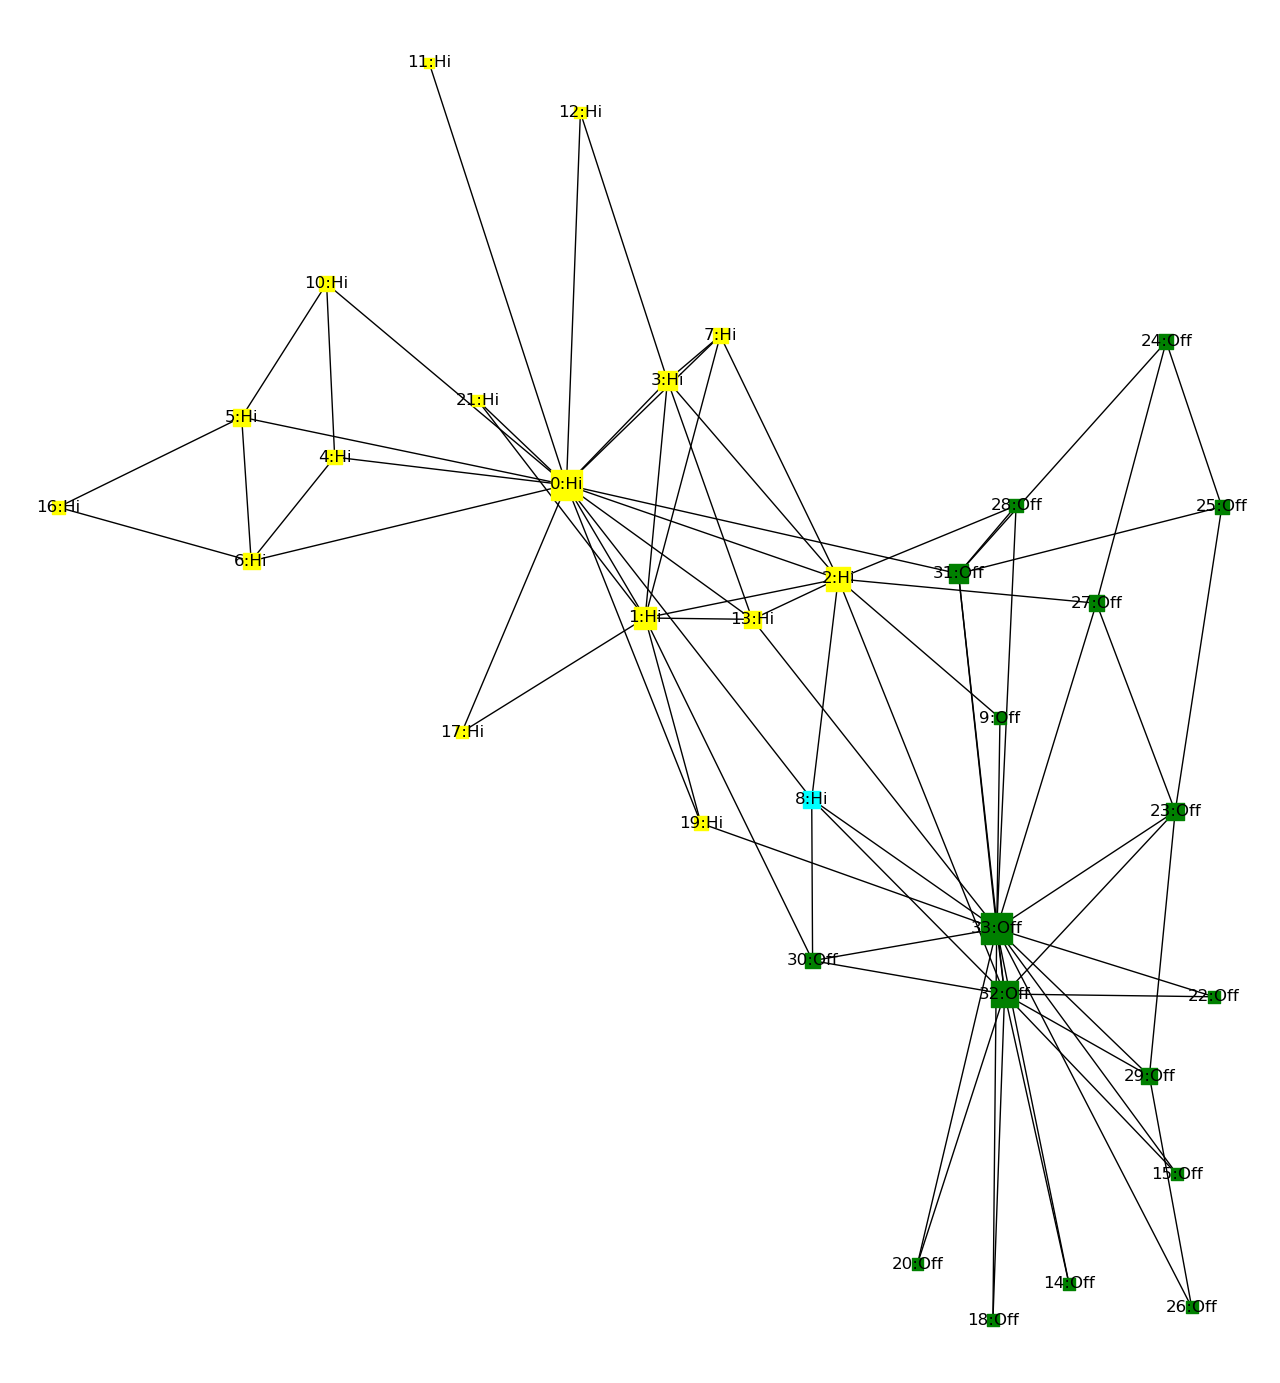
\includegraphics[width=0.75\linewidth]{Karate_coolwarmclustering.png}
\caption{
The Famous 'Zachary's Karate Club' Graph. The labels show the actual division
between the 'Mr Hi' and 'Officer' groups.
Vertex size indicates its PageRank.
The colors encode the result of the coolWarmClustering compared to the actual
partition. It made 1 mistake:
It associates wrongly vertex 8 to 'Officer'.  This vertex
is hard to resolve because it is connected to hubs in both clusters.
In fact a further check confirms that the total sum of 'heat' it sends to members of
'Officer' is $0.45$ vs $0.36$ to members of 'Mr Hi' (excluding itself in both
cases). So in some sense the algorithm is more correct then the actual
partition in real life. Perhaps this is due to human irrationality?
On the other hand, $8$ receives more heat units from $17$ members of 'Mr. Hi': $0.485$
units, compared to $0.345$ units from the $16$ members of 'Officer'. 
}
\label{fig:karatecoolwarm}
\end{figure}

\begin{figure}
\centering
\begin{subfigure}[b]{0.5\textwidth}
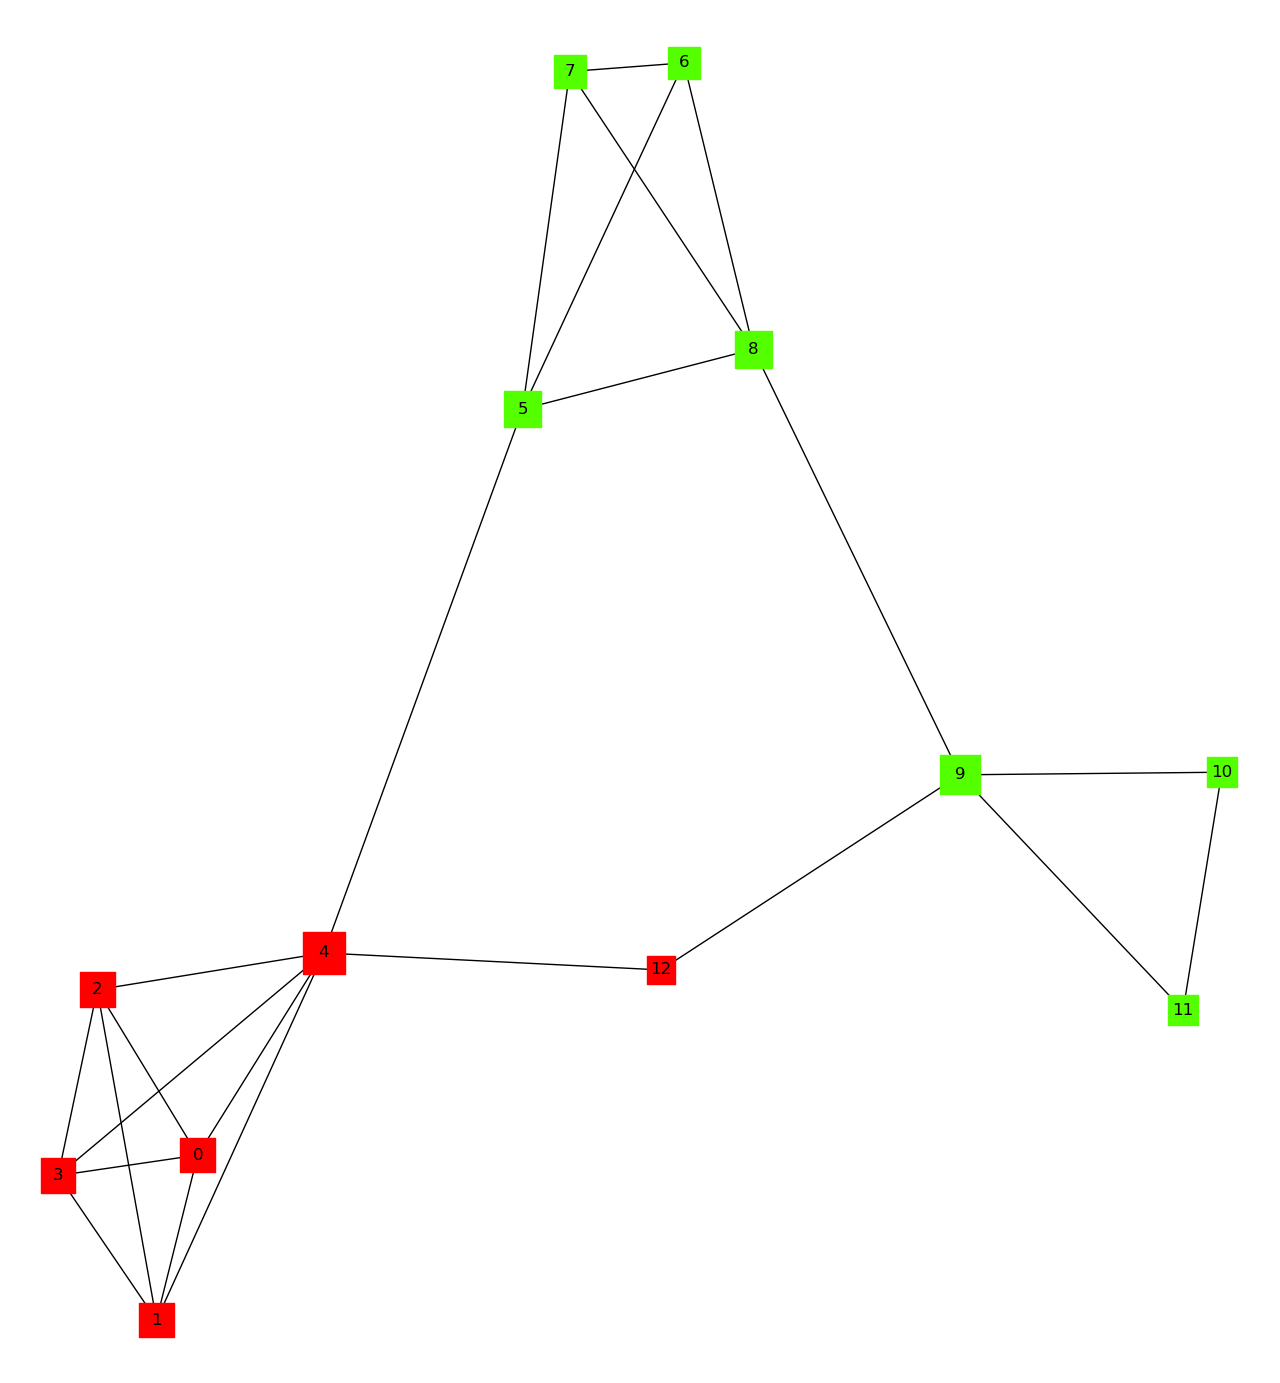
\includegraphics[width=\textwidth]{example_coolwarm2clusters.png}
\caption{A 2 cluster partition}
\label{fig:examplecoolwarm2cluster}
\end{subfigure}
%add desired spacing between images, e. g. ~, \quad, \qquad, \hfill etc. 
%(or a blank line to force the subfigure onto a new line)
\begin{subfigure}[b]{0.5\textwidth}
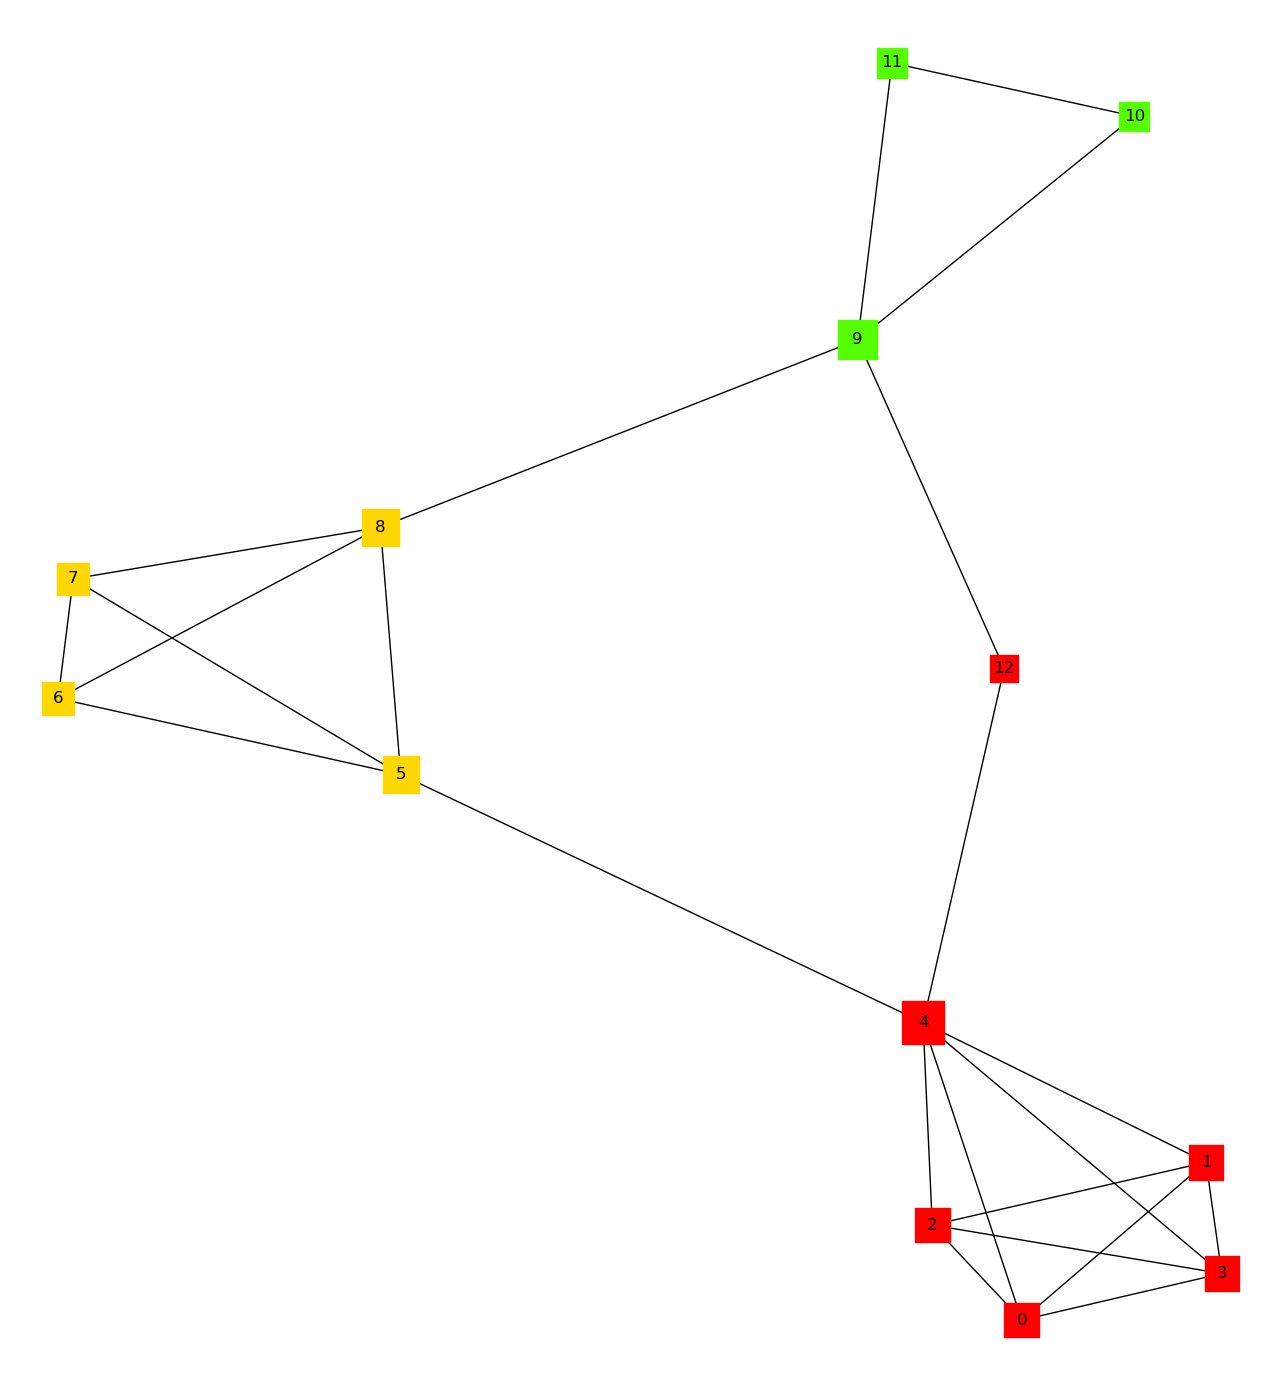
\includegraphics[width=\textwidth]{example_coolwarm3clusters.png}
\caption{A 3 cluster partition}
\label{fig:examplecoolwarm3cluster}
\end{subfigure}
%add desired spacing between images, e. g. ~, \quad, \qquad, \hfill etc. 
%(or a blank line to force the subfigure onto a new line)
\caption{The result of running the algorithm set for finding a 2-partition and
respectively a 3-partition. The interesting node is 12. In both runs 12 chooses
to associate with the biggest clique because node 4 of that clique is the one
which receives the most heat from 12}
\label{fig:exampleCoolWarmClustering}
\end{figure}



\section{Spectral clustering and other methods}

\textbf{Spectral Partitioning} 
\cite{von2007tutorial, naumov2016parallel, WikipediaGraphPartition, WikipediaSpectralClustering},
is a common technique for partitioning graphs. The idea is to construct a
Laplacian type matrix \cite{WikipediaLaplacianMatrix} for the graph $G$ and
analyze its eigenvalues and eigenvectors and construct a $2$-partition of $G$.
It is possible to create a hierarchical partitioning of $G$ by repeating the
process on each subdivision.

The problem of finding the best graph partition, also called the minimal cut
problem is NP-hard. Spectral partitioning methods are heuristics that
approximate the solution in 'real life' classes of networks.

\begin{mydef}
\label{def:Laplacian}
Let $G$ be a bidirectional graph with adjacency matrix $A$ and diagonal degree
matrix $D$.
Then the following matrices are its \textbf{graph Laplacian}, and its
\textbf{symmetric\textemdash
, row\textendash normalized\textemdash and column\textendash normalized\textemdash Laplacians}:  

\begin{equation}
\begin{aligned}
L & = D - A \\
L_s & = D^{-1/2}LD^{-1/2} = I - D^{-1/2}AD^{-1/2} \\
L_r & = D^{-1}L = I - D^{-1}A \\
L_c & = LD^{-1} = I - AD^{-1}
\end{aligned}
\end{equation}
\end{mydef}

Consider the connected graph $G$ and its adjacency matrix $A$. We create the transition
matrix by normalizing it: $T = AD^-1$, and finally we choose a restart parameter
$\alpha$ and create the diffusion kernel $K$. Theorem
\ref{thm:AKTcharacteristics} assures us that $K$ and $T$ have the same
eigenvectors and the orders of their corresponding eigenvalues are the same. The
eigenvalues are all real and therefore the eigenvectors are real as well. And
the eigenvalues of $K$ are all non-negative.

The matrix $K^{-1} = \alpha^{-1} [I - (1- \alpha) AD^{-1}]$ is closely related to the
and the column-normalized Laplacian $L_c$. The added parameter $0 \lt \alpha \lt 1$
neither changes the eigenvectors, nor the order of the corresponding eigenvalues.

The smallest eigenvalue ,$0$ of $L$ and $L_s$
corresponds to the largest eigenvalue $1$ of and $T$ and its eigenvector is
(can be chosen as) all positive. 
Any other eigenvector of $L$ (which corresponds to an eigenvector of $T$) must
contain both positive and negative components due to \ref{thm:perron1}.

It's the eigenvector of the second smallest
eigenvalue $L$ or $L_s$ which is commonly used in 
They are commonly referred to as the \textbf{Fiedler} eigen-pair in the literature.
for spectral partitioning \cite{naumov2016parallel}. The simplest method is to
use the sign of the components of
eigenvector of the second smallest eigenvalue of $L$ or $L_s$.
This eigen-pair corresponds to the second largest eigenvalue of $T$

In \textcite{newman2006modularity} there is a particular type of spectral
partitioning which uses a matrix which the author called the modularity matrix.
It has the advantage over the Laplacian in that its greatest eigenvalue may be
positive or negative which is used to indicate or suggest the existence of
community structure in the graph. However the normalized Laplacians $L_r$ and
$L_c$ are more natural in the context of the random walk or propagation method
and recommended for example in \cite{von2007tutorial}.


\begin{figure}
\centering
\begin{subfigure}[b]{0.5\textwidth}
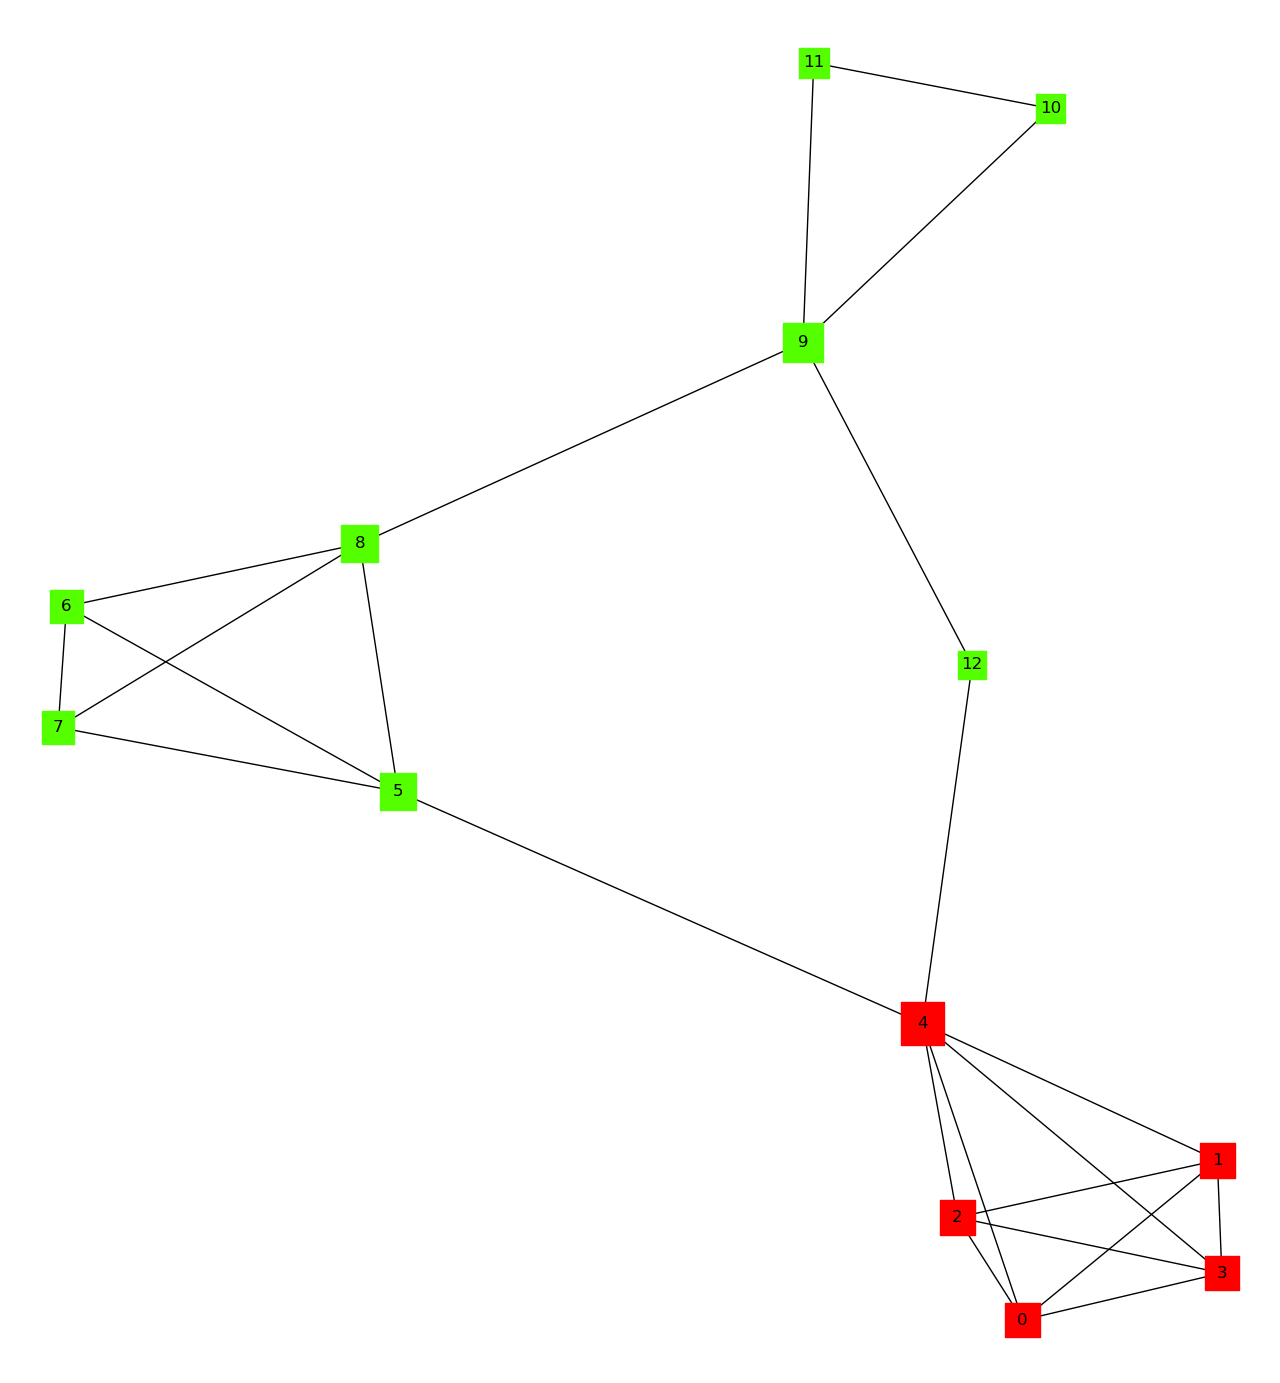
\includegraphics[width=\textwidth]{example_spectralT2clustering.png}
\caption{A spectral clustering using the sign of the Fiedler eigenvector.}
\label{fig:toygraphspectralclustering}
\end{subfigure}
%add desired spacing between images, e. g. ~, \quad, \qquad, \hfill etc. 
%(or a blank line to force the subfigure onto a new line)
\begin{subfigure}[b]{0.5\textwidth}
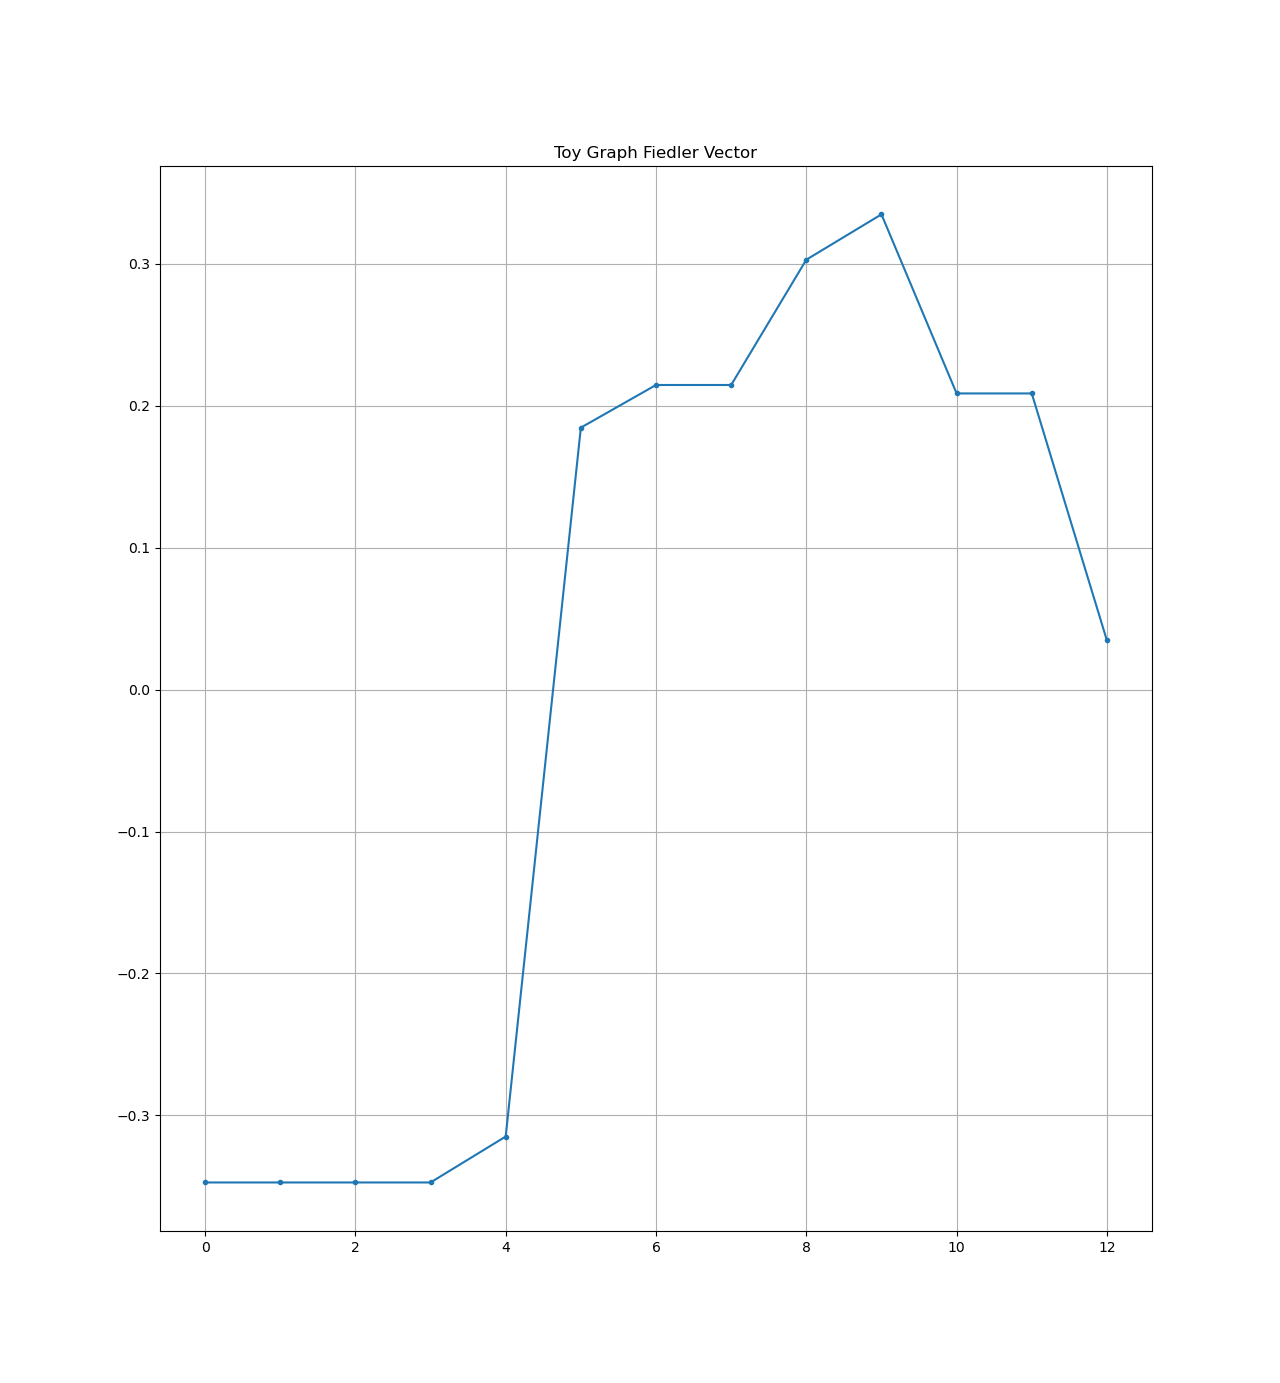
\includegraphics[width=\textwidth]{Toygraph_Fiedler.png}
\caption{Plot of the Fiedler vector's components, showing a clear subdivision
between the positive and the negative components.}
\label{fig:toygraphfiedlerplot}
\end{subfigure}
%add desired spacing between images, e. g. ~, \quad, \qquad, \hfill etc. 
%(or a blank line to force the subfigure onto a new line)
\caption{}
%\label{fig:exampleCoolWarmClustering}
\end{figure}

\begin{figure}
\centering
\begin{subfigure}[b]{0.5\textwidth}
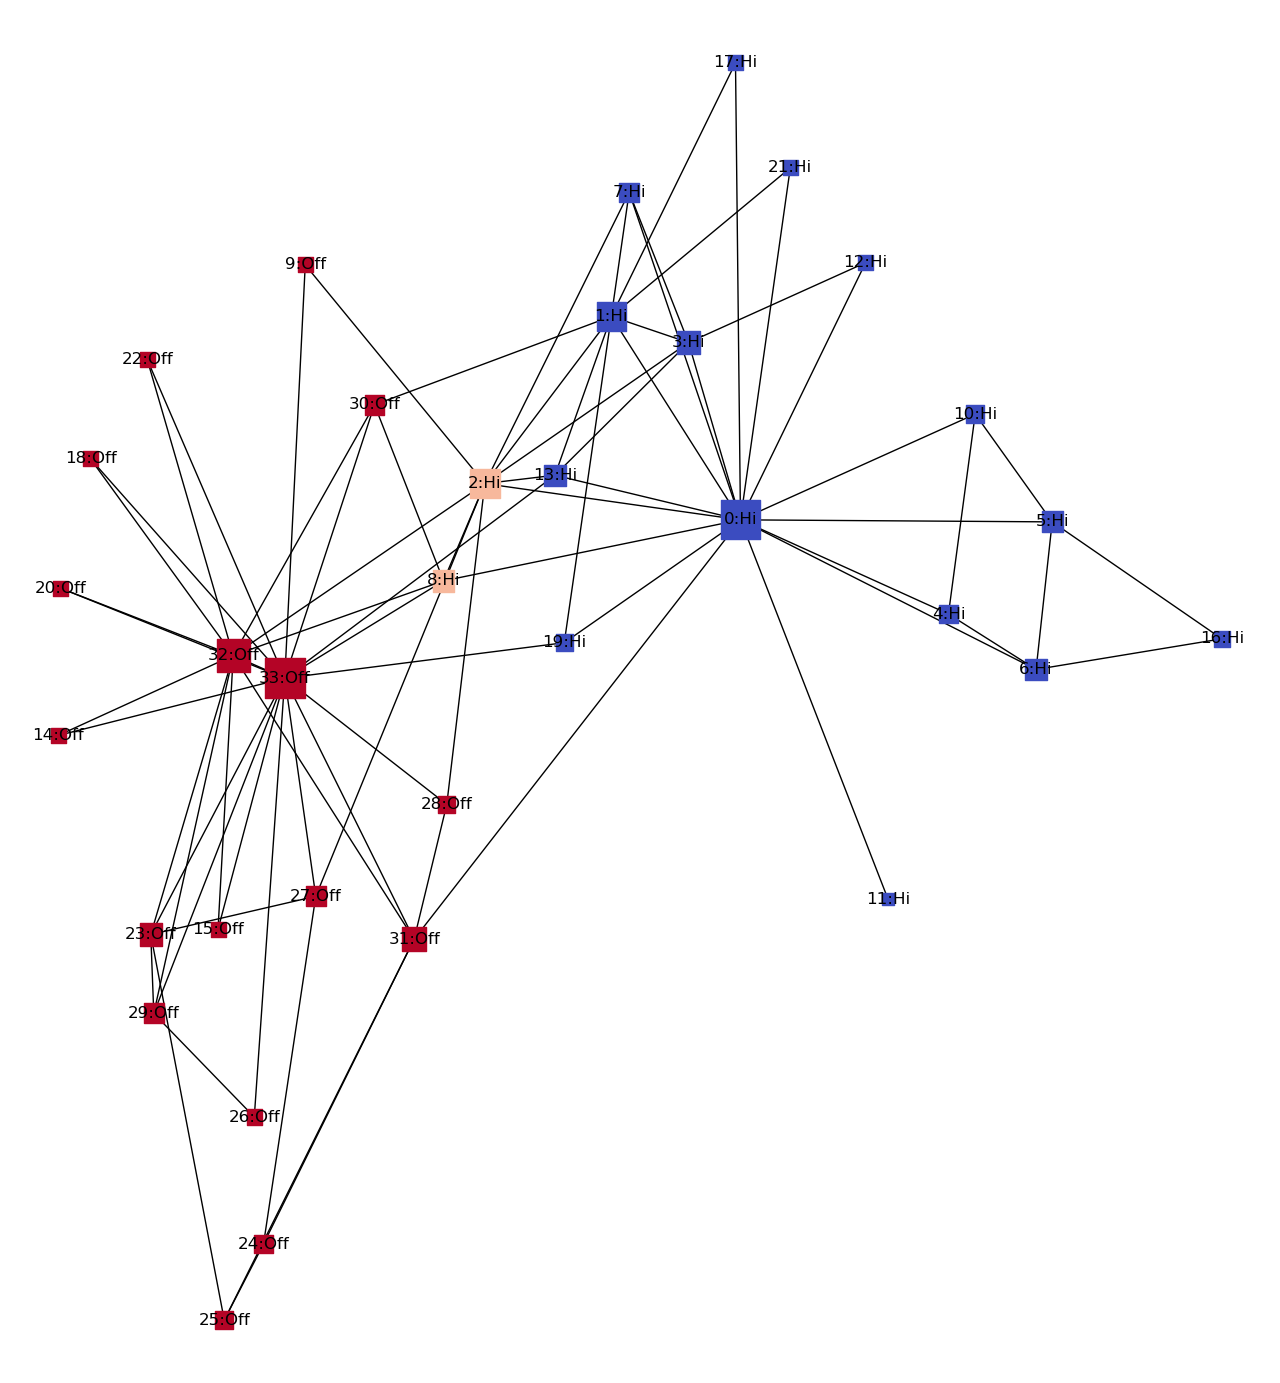
\includegraphics[width=\textwidth]{Karate_spectralT2clustering.png}
\caption{Spectral clustering of the Karate Club network using the Fiedler
eigenvector signs. There are $2$ deviations from the actual partition, both are
borderline nodes which are harder to resolve. The $8$ node mistake is in common
with the naive algorithm of the previous section.}
\label{fig:karatespectral}
\end{subfigure}
%add desired spacing between images, e. g. ~, \quad, \qquad, \hfill etc. 
%(or a blank line to force the subfigure onto a new line)
\begin{subfigure}[b]{0.5\textwidth}
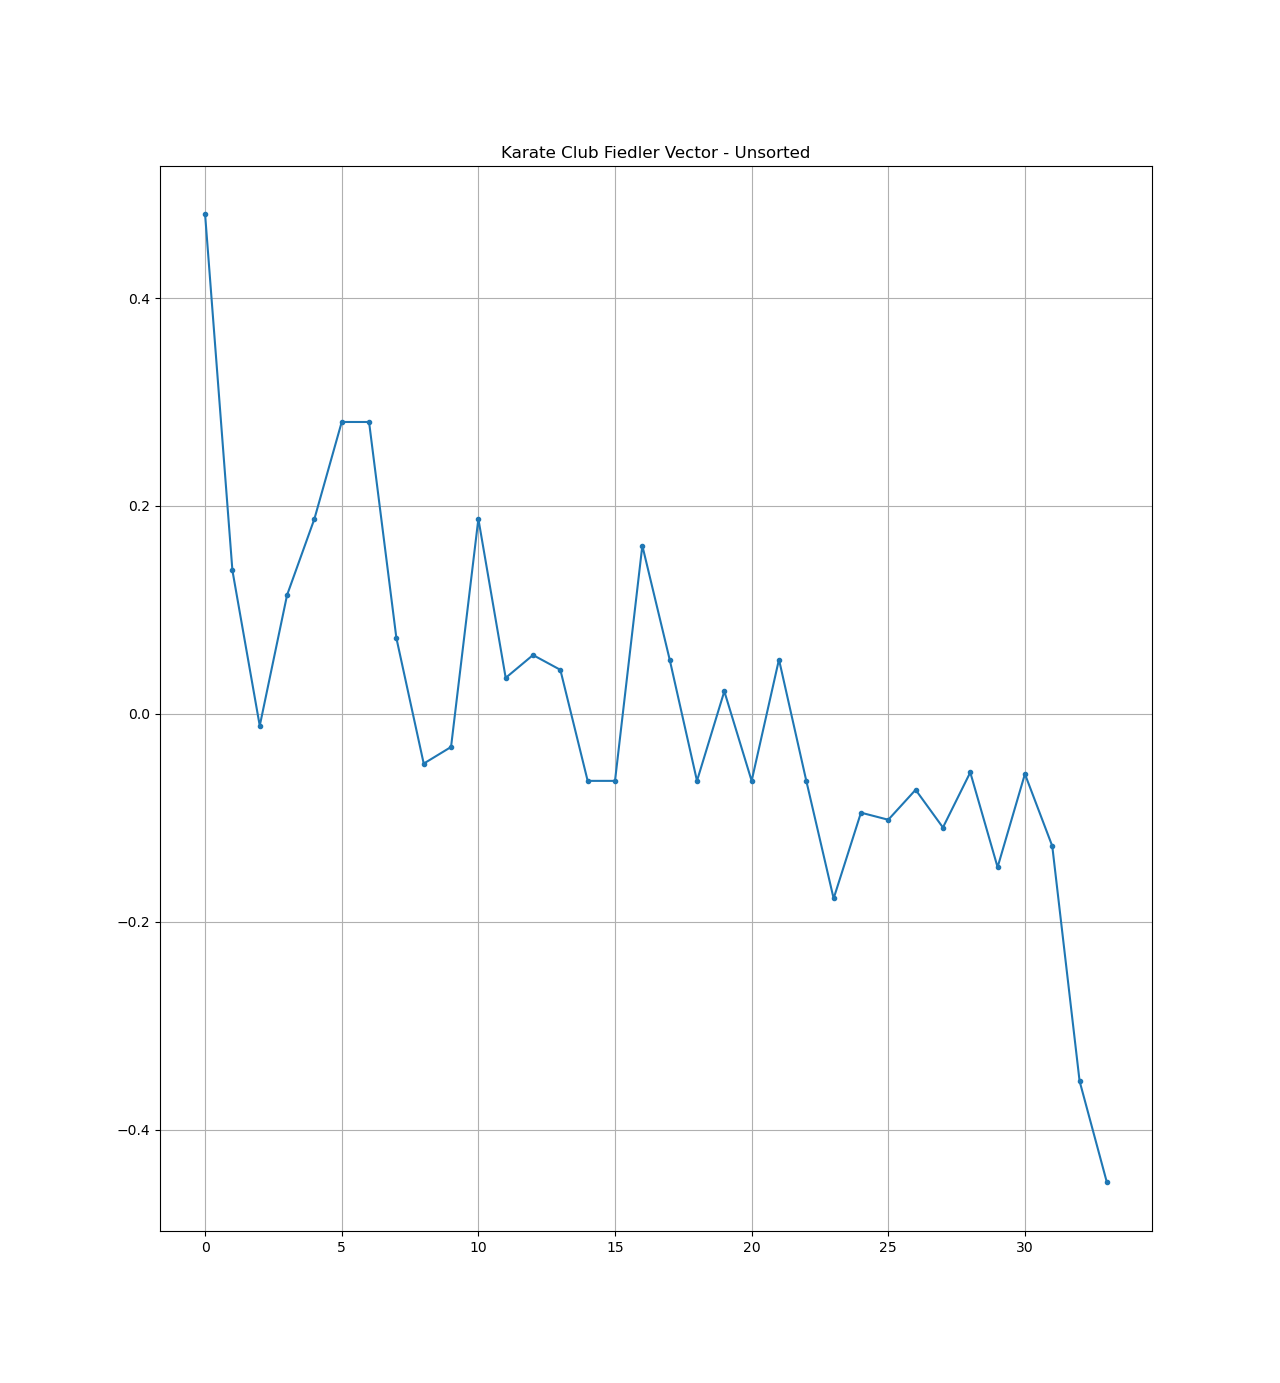
\includegraphics[width=\textwidth]{karate_fiedler_unsorted.png}
\caption{Plot of the Fiedler Vector of the Karate Club. The split between
negative and positive values is much less dramatic but nonetheless still visible.}
\label{fig:karatefiedlerplot}
\end{subfigure}
%add desired spacing between images, e. g. ~, \quad, \qquad, \hfill etc. 
%(or a blank line to force the subfigure onto a new line)
%\caption{}
%\label{fig:exampleCoolWarmClustering}
\end{figure}

\section{(Trying) function prediction method}
In this section we are going to try to apply the accumulated knowledge of the
previous sections and devise some simple function prediction algorithms for PPI
networks. We are going to try several methods which use propagation as well as
methods which just use direct neighbors for the predictions.

The network is going to be composed of around 500 vertices (proteins) which are
divided into 4 different function groups. We are going to randomly choose half
the proteins and mark them as unknown and try to predict their function based
on the remaining known proteins. 

\subsection{Methodology}
We use the annotated yeast interactome which is a pure PPI network that comes
prepackaged with the
software tool 'Cytoscape'. The nodes represent yeast proteins and the edges
represent protein-protein interactions.

This network comes with functional annotations in the 'MCs name' field. We
select nodes in the network whose annotations contain \textbf{exactly} one
of the following
keywords:  'DNA Replication' (blue group), 'Golgi' (red), 'Meiosis' (yellow),
and 'Stress response' (green). All other nodes are removed from the network.
The result is shown on figure \ref{fig:yeast_subgraph_4groups}. We are going to
test various annotation method on the largest connected component of this
subnetwork.

Nodes whose annotations contain keywords of more then one group were discarded.

\begin{figure}
\centering
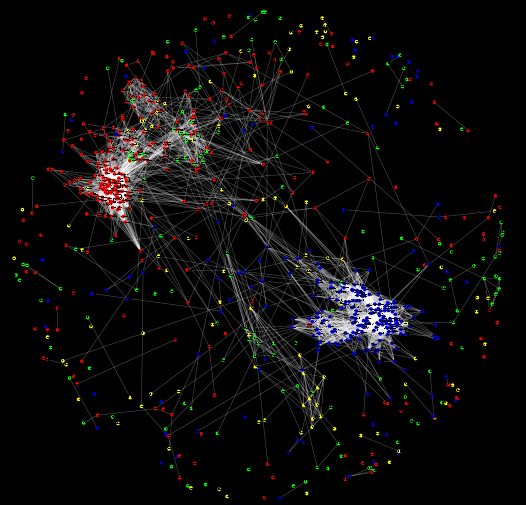
\includegraphics[width=\textwidth]{yeastsubgraph_4_groups_colorcode.png}
\caption{Subgraph of the yeast interactome showing nodes of 4 groups: 'DNA
replication' (blue), 'Golgi' (red), 'Meiosis' (yellow), 'Stress response'
(green)}
\label{fig:yeast_subgraph_4groups}
\end{figure}

The above described subnetwork is exported from cytoscape to graphml file, which we import 
and convert into a networkx object. 
We select the largest connected component from the above network.

We set a random seed (a process which we repeat 2 times for 2 different trials).
Then we select randomly 50\% of the nodes and mark them as 'unknown'. The other
50\% are 'known'. We are going to try to determine the group affiliation of the
unknown nodes based on the group affiliations of the known nodes.

We use 5 different prediction methods:

\begin{itemize}
\item{Method 1} Determines the group affiliation of an unknown node by the group
that has the maximal volume based on the propagation distribution from the
unknown node. This meas: we calculate the stationary distribution with restart
to the unknown node. Among the known nodes, we calculate the weighted sums of
each of the 4 groups according to that distribution. The group with largest
volume is the affiliation we assign to the unknown node.

\item{Method 2} This method works like method 1, except that we first order the
unknown nodes (decreasing order) according to their pageRank. We go over the
nodes in this order and assign group affiliation according to method 1, but then
we also update the list of the known nodes to include that node. So this node is
going to be included in the function prediction of the lower ranked nodes.

The rational here is that the higher ranked nodes are probably going to be
predicted with high accuracy and therefore be helpful in prediction of lower
ranked nodes. 

It is probably better to device some simple rule to decide whether it is worth
to include a node in the prediction of the rest of the nodes. For example, based
on how many unknown neighbors in has vs known neighbors. But we tried to keep
things simple at this stage.

\item{Method 3} We assign an unknown node to the group that has plurality among
its neighbors with known group affiliation. So this method is fast and the
probably the simplest.

\item{Method 4} Same as method 3, but again we go in the order of pagRanks and
we update the list of known nodes on the fly, like method 2.

\item{Method 5} Here we take each group of the known nodes and propagate from
it. So for example we calculate the stationary distribution when we restart in
the known nodes that belong to group 'DNA Replication', and then for the next
group and so forth. For each unknown node, we assign it to the group that
propagates the highest probability to it.

So while in method 1 and 2, we start random walking from an unknown node and see
what is the probability that we land at a certain group. In Method 5 we start
walking randomly from one of the members of a group and check what is the
probability that we visit a certain unknown node.

This method is an order of magnitude faster than method 1 and 2 because we only
need to calculate the stationary distributions 4 time (pageRank and for each
group). However we suspect it will perform with less accuracy.
Because they take into account nodes that are far and not well connected to the
unknown node whose function we try to predict.
The function groups, in particular the yellow (meiosis) and green (stress) are not
well clustered and spread all over the network.

\end{itemize}

\subsection{Somew code snippets}
\begin{lstlisting}[language=python]
# The decision function which is used in methods 1 and 2 to predict a single
# node
def decision_function(v, G, group_membership_ar, known_unknown_ar):
    """Input v: an node assumed to be an int and taken from the list of unkown
    nodes. Input G: The graph. 
    Input group_membership_ar: Array of strings which specifies for each node 
    to which group belongs (including the 'unkonw' nodes) this is required for
    thesting the correctness of the decision.
    Input known_unknown_ar: boolean 1d array which
    specifies for each node of the graph whether its membership is known or
    unkown. 
    output guess_group: string the group that the function assigns the node to.
    output correctness: True or false depending on the correctness of the
    guess_group vs the real group_membership_list[v] value.
    """
    all_nodes = np.arange(len(G.nodes))
    known_nodes = all_nodes[known_unknown_ar]
    unkown_nodes = all_nodes[known_unknown_ar == False]
    bias = np.zeros_like(G.nodes)
    bias[v] = 1
    bias
    p = biasedPropagateGv2(G, bias=bias)
    group_names = np.unique(group_membership_ar)
    q = p * known_unknown_ar #0 on all unkown nodes
    testscores = np.zeros_like(group_names)
    for g in range(len(group_names)):
        x = q[group_membership_ar == group_names[g]] 
        testscores[g] = x.sum()
    decide = group_names[np.argmax(testscores)]
    correctness = decide == group_membership_ar[v]
    return decide, correctness

# Main part of method 2:
# Which is actually similar in methods 1-4
known_unknown2 = known_unknown.copy()
node_colors2 = node_colors.copy()
score2 = 0
for v in orderedUnkownNodeList:
    _, test = decision_function(v, G, groups, known_unknown2)
    score2 += test
    known_unknown2[v] = True #mark v as 'known'
    G2.nodes[v]['correctness2'] = "Correct"
    node_colors2[v] = 'brown'
    if not test: # mark as incorrect and colormark if mistake
        node_colors2[v] = 'pink'
        G2.nodes[v]['correctness2'] = "Mistake"
\end{lstlisting}

%\begin{figure}
%\centering
%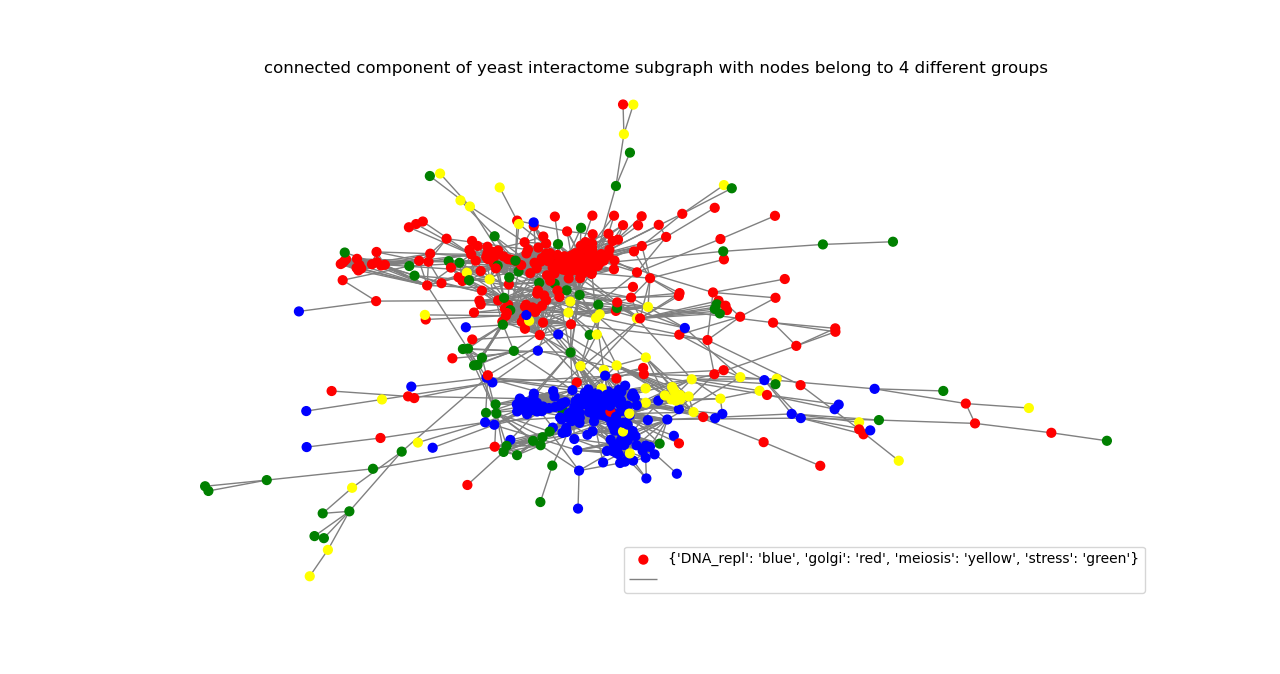
\includegraphics[width=\textwidth]{connected component of yeast interactome subgraph with nodes belong to 4 different groups.png}
%\caption{The largest connected component which was selected for the function
%prediction experiment. Here the Correct group affiliation of all nodes is color
%coded.}
%\label{fig:largest_connected_comp}
%\end{figure}

\subsection{Results}

\begin{table}[!htb]
\caption{Prediction Accuracy of the 4 Methods in 2 different random
trials. Each trial with a different seed, which result in different randomly
selected known/unknown nodes.} 
\begin{center}
\begin{tabular}{ | l | c | c | c | c | c | }
\hline
Seed / Method & 1 & 2 & 3 & 4 & 5\\
\hline
42 & 0.795 & 0.858 & 0.765 &
0.784 & 0.701\\
6382020 & 0.774 & 0.832 & 0.752 & 0.748 & 0.755\\
\hline
\end{tabular}
\label{table:results_5_prediction_methods}
\end{center}
\end{table}

\begin{figure}
\centering
\begin{subfigure}[b]{\textwidth}
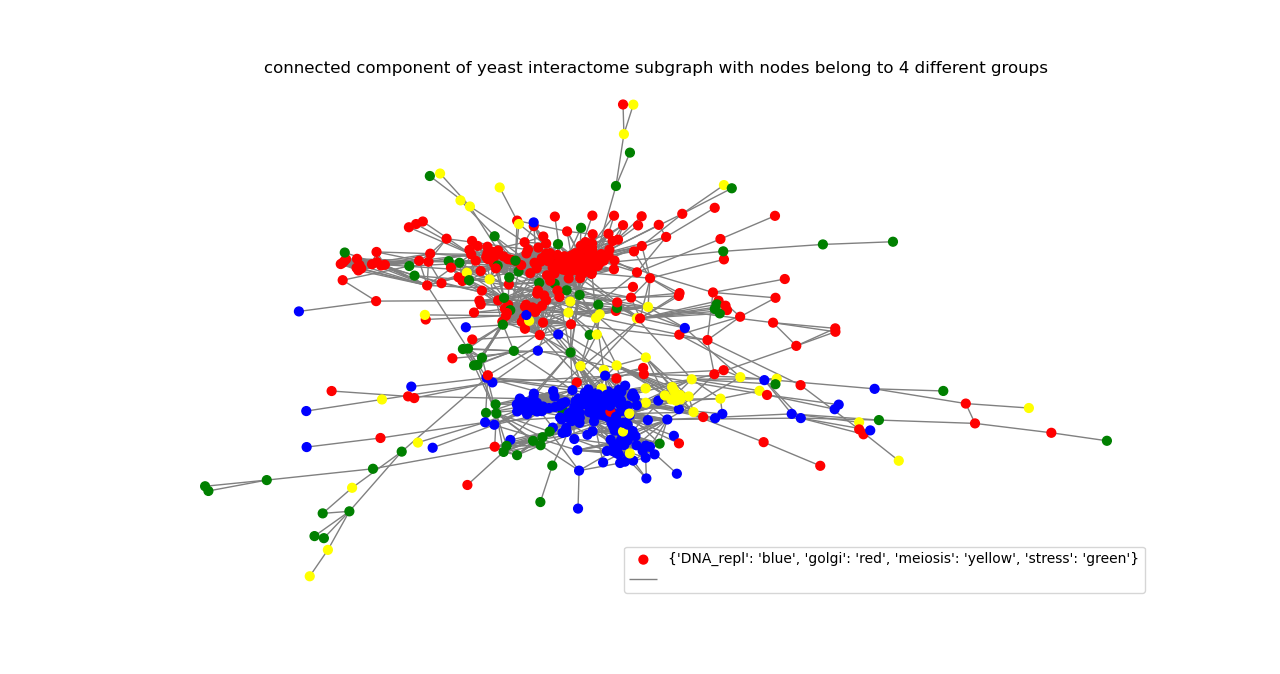
\includegraphics[width=\textwidth]{connected component of yeast interactome subgraph with nodes belong to 4 different groups.png}
\caption{The largest connected component which was selected for the function
prediction experiment. Here the Correct group affiliation of all nodes is color
coded.}
\label{fig:largest_connected_comp}
\end{subfigure}
\begin{subfigure}[b]{\textwidth}
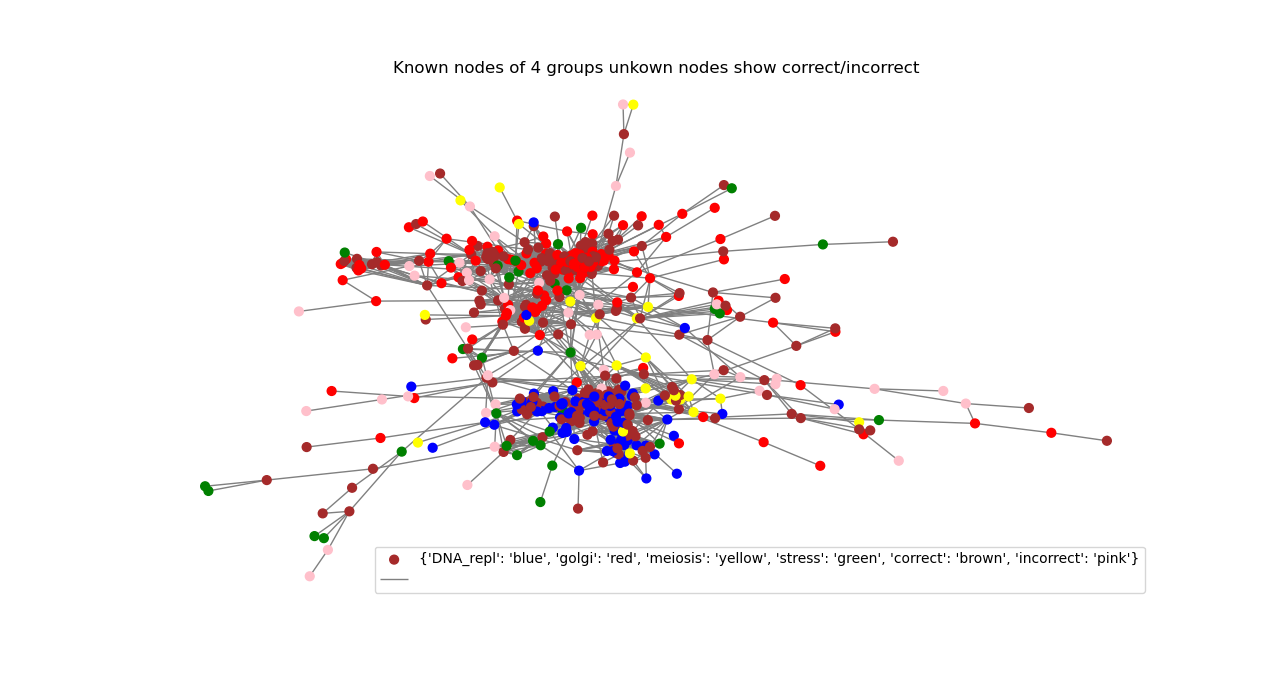
\includegraphics[width=\textwidth]{method2_true_false_clustering_on_4_groups_with_ordering_and_update.png}
\caption{The result of predictiob method 2, which was the best perfomer. 
The known groups are color coded by RGBY. The unkown nodes are color
coded: brown:correct prediction, pink:incorrect.}
\label{fig:my_prediction}
\end{subfigure}
\end{figure}

\subsection{Discussion}
If we look at figure \ref{fig:largest_connected_comp} which shows the connected
component that we worked with, the red and blue are pretty nicely clustered. The
The greens and specially the yellows are sort of spread all over the network and
not nicely clustered. I don't know if this is a good example of a real world
scenario.

When we look at figure \ref{fig:my_prediction} it seems that most of the
incorrect predictions are on nodes that seem 'peripheral' and  are not well
connected to known nodes. Another source of mistakes seems to bee green nodes
that are too close to the red cluster.

Method 2 shows somewhat higher accuracy over the other methods but on the flip
side it is an $O(n^2)$ method when optimized methods are used whereas methods
3,4,5 are $O(n)$.

It's probably woth while to repeat the experiment a couple of hundred of times
to estimate the mean accuracies of the methods.


\section{The Propagation Method In Bioinformatics}
%The normalize adjacency matrix of 
%a connected graph (for simplicity we use here undirected) is a transition matrix
%and represents a
%Markov process. On a given time-step, a visitor on a graph node chooses
%his next station at random among the neighbours of the current station (node).
%
%We want to know first, if we repeat this process to infinity will the frequency
%of the visits at each node stabilizes.

%\lipsum[3-4]

Propagation methods or as they are sometimes called, diffusion methods, have
been used in Bioinformatic software tools mostly function prediction and
'disease characterization' \cite{cowen2017network}.

Typically the diffusion method is used to screen for possible 'candidates' (i.e
a disease causing genes) which is basically pageRanking, or for module detection
which is essentially clustering/community structure. In a second step these
candidates are scored by a probabilistic model which may use additional
information beyond the network structure itself.

The most simple application, which is briefly described in the introduction, is 
function prediction in a single PPI network. As an example application we bring
the RIDDLE \cite{wang2012riddle} functional prediction web application
(\url{www.functionalnet.org/RIDDLE}). 

(usw und sofort \dots they use pagrRank, and then do a statistical test based on
hypergeometric distribution to score the significance \dots) 




Hotnet \cite{vandin2012discovery} and its successor Hotnet2
\cite{leiserson2015pan} are an example of a more complex application
used for module detection \dots

(they have a system to set threshold influence, break the graph to small 
connected components as module candidates, then use additional information 
to score the significance)


\begin{comment}
\section{testing}

\subsection{citations}

For more info see (textcite) \textcite[631]{meyer2000matrix}.

This is a normal (cite)~\cite[p.~115]{big}.

This is an (autocite) see \autocite[231]{lion2010}.

Change autocite in the usepackage definition to suit your needs. Use textcite if
you want to insert inline cite that includes the author's name.

Here is a~\cite{WikipediaPerronFrobenius} cite from wikipedia.

Just cite is just the normal citation command and nocite will make sure that the
reference appears in the bibliography even though it may have not specifically
been mentioned in the text somewhere.

\subsection{Images}

Here is an image

%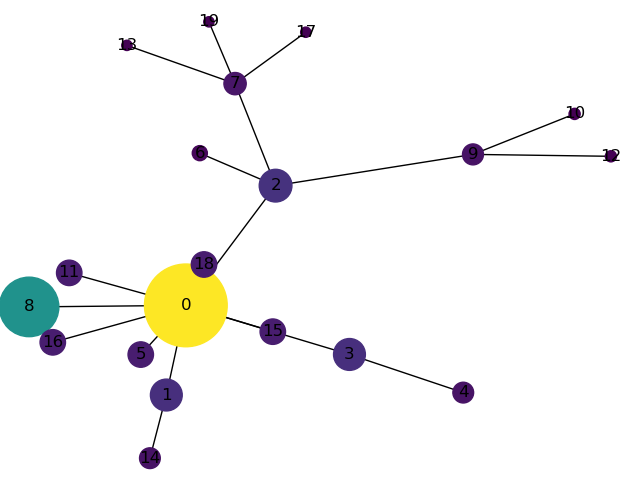
\includegraphics{BA20-1.png}

\begin{figure}[!htb]
  \centering
    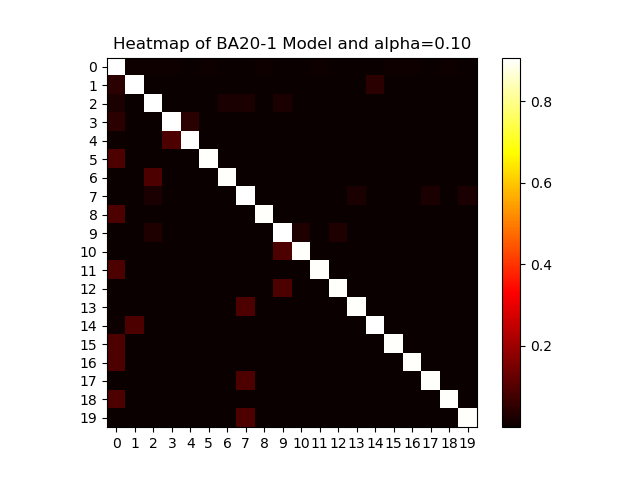
\includegraphics[width=0.65\linewidth]{Heatmap BA20-1 alpha=0.10.png}
  \caption{Heatmap. Alpha=0.1}
  \label{fig:heatmap}
\end{figure}

Refer to it with fig \ref{fig:heatmap} tada.


\begin{figure}[!htb]
  \centering
    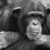
\includegraphics[width=0.65\linewidth]{test2.png}
  \caption{The apparatus used in the experiment. The forward right
  wing is fixed to the chain wheel which controls its elevation.
  The electrodes sticking out of the black precision clamp 
  are positioned to touch the exposed meso N1 at the root of the
  wing}
  \label{fig:apparatus}
\end{figure}

\subsection{Tables}

\begin{table}[!htb]
  \caption{Nernstsche Gleichgewichtspotenziale und das resultierende
  Membranpotenzial nach Goldmann Gleichung} 
\begin{center}
  \begin{tabular}{ | l | c | c | c | c | }
    \hline
     Ion & rel' Permeabilität &  Konz. in & Konz. auß & GG
     Potenzial \\ \hline
     $K^+$ & 1 & 124 & 4 & -86.74 \\
     $Na^+$ & 0.04 & 50 & 470 & 56.6 \\
     $Cl^-$ & 0.3 & 55 & 580 & -59.51 \\
    \hline
    $V_m$ &
    \multicolumn{4}{ | c |}{-51.35} \\
    \hline
  \end{tabular}
  \label{table:amp/dauer}
\end{center}
\end{table}

\end{comment}

\section{Reference}
\nocite{slides_from_lecture}
\nocite{cowen2017network}
\nocite{vandin2012discovery}
\nocite{vandin2012discovery}
\nocite{leiserson2015pan}

\printbibliography

\end{document}
